\documentclass[12pt]{article}
\usepackage[utf8]{inputenc}
\usepackage{amssymb}
\usepackage{amsmath}
\usepackage{textcomp}
\usepackage{graphicx}
\usepackage[a4paper, portrait, margin=1in]{geometry}
\usepackage[capposition=top]{floatrow}
\usepackage{longtable}
\usepackage{booktabs}
\usepackage{setspace}
\usepackage[style=authoryear,backend=biber,sorting=nyt]{biblatex}
\addbibresource{references.bib}
\usepackage{pdflscape}
\usepackage{indentfirst}

\doublespacing
\begin{document}

\begin{titlepage}
	\begin{center}
		\vspace*{2cm}
		
		\large
		The Subprime Crisis Revisited: Unpacking the Long-Term Performance of a 2007 Bear Stearns Mortgage-Backed Securities Deal
		
		\vspace{2cm}
		
		\large
		Alex Blumenfeld\footnote[1]{Boston University and Chicago Booth; alex.blumenfeld@chicagobooth.edu. Funding for this project was provided by Boston University's Undergraduate Research Opportunities Program, and by Robert King of the Boston University Department of Economics.}
		
		\text{November 11, 2023}
		
		\vspace{1cm}
		
		\begin{abstract}
\noindent Residential mortgage-backed securities (RMBS) came under intense public scrutiny in the wake of the 2007 financial crisis and the subsequent Great Recession, but have since lost their status as a significant political issue. In order to provide some anecdotal answers about whether these securities were truly as dangerous as many came to suspect during the crisis, I engage in a ``postmortem'' on one particular securitization which was issued shortly before the financial chaos of 2007: Bear Stearns Asset-Backed Securities 2006-HE10. I find that out of an original principal pool of roughly \$1.1 billion, 44.2\% of the total principal from the deal’s mortgages has been written off due to defaults, but thanks to the deal’s credit enhancement mechanisms, investors have felt only 50.6\% of these losses, giving them a principal loss rate of 23.5\% through March 2020. As for the underlying mortgages, I find that foreclosures did not peak until around 2012, showing that security principal markdowns which occurred during the financial crisis itself did not capture the full extent of the mortgages’ poor performance. I also focus on two senior tranches which were purchased by the Federal Reserve’s Maiden Lane fund in 2008, when the Fed agreed to buy seemingly toxic RMBS from Bear Stearns’s portfolio to facilitate the firm’s sale to JPMorgan Chase. One of these tranches has suffered only modest principal losses, and the other has had no principal losses whatsoever, suggesting that little in-depth analysis of these securities was conducted during the height of the crisis.
		\end{abstract}
		
		\vfill
		
	\end{center}
\end{titlepage}

\section*{Introduction}

The history of the modern notion of securitization begins in 1970, when the very first mortgage-backed security (MBS) was created, and in the half-century since then, this practice has built its own unique niche in the global financial markets. It all began when the Government National Mortgage Association (a.k.a. Ginnie Mae) began bundling together the mortgages it issued and selling securities which had the right to collect the cash flows from those mortgages, complete with a guarantee that the U.S. government would reimburse investors for missed principal and interest payments \parencite{segoviano13}. Although advancement in this nascent field was slow at first due to regulatory complexity and a dearth of high-powered computers needed for many related calculations, securitization took off exponentially in the 1990s, and before long, a much wider variety of assets, from non-government-issued mortgages to credit card bills to auto loans, were being securitized. As banks saw that they could use securitization to lower their costs of funding – because borrowing in the global capital market by selling the rights to collect cash flows from a group of loans was generally cheaper than borrowing from a single source – they became eager to securitize everything they could. The massive “conventional” mortgage market, which refers those mortgages which are not originated by a government-sponsored enterprise like Ginnie Mae or Freddie Mac, was the main target of these efforts, because most of these loans were being made by small banks which charged relatively high rates on mortgages, seemingly due to their lack of access to funding from global markets \parencite{brendsel98}. Of course, these securities no longer had government guarantees to entice investors, so issuers were forced to get more creative with methods of protecting investors’ capital against losses, and investors also began to apply more sophisticated methods in their evaluation of these non-guaranteed MBS. Supply and demand for MBS and other securitized products both continued to grow, as banks discovered the financial benefits of packaging and selling their loans, and a wide variety of investors became hungry for both high-yielding mezzanine tranches and safer senior-level securities.

Unfortunately, these sell-side and buy-side forces combined to put pressure on the incentive structure of the securitization process, and underwriting standards for non-government-guaranteed MBS began to slip in the late 1990s and early 2000s. Whereas in the past all mortgages included in MBS loan pools were required to conform to the standards of Freddie Mac or a similar agency, this requirement was thrown out the window in the subprime market, and the quality of the underlying collateral on many deals began to drop compared to that of past securitizations. \textcite{segoviano13} describe this as one step in a “self-reinforcing credit intermediation cycle”, where a monetary incentive to securitize as many loans as possible in order to meet demand for MBS leads to weak underwriting standards, and then the complex securitization process convinces investors that these questionable loans can be combined to form a high-quality asset, boosting the demand for these attractive securities. From here, it’s not hard to imagine the markets falling further down this slippery slope: when the U.S. housing market topped out in 2007 and subsequently crashed, the formerly bulletproof mortgage-backed securities that had been flooding the market suddenly didn’t look so attractive. After the dust settled, the banks which had engaged in the opaque process of securitization, along with the credit rating agencies that assigned AAA ratings to securitizations full of poorly performing loans, found themselves saddled with much of the blame for allowing the financial system to approach abject collapse.

Now, over a decade after the credit crunch and bank bailouts of 2007 and early 2008, we will attempt to understand the legacy of securitization in the context of the Great Recession by breaking down one specific deal that fits perfectly into the trends we’ve discussed so far: Bear Stearns Asset-Backed Securities (BSABS) 2006-HE10. Consisting of just over \$1B of mortgages issued just before the financial crisis, this particular deal makes a great choice for the kind of analysis done here. Among other reasons, data on its historical cash flows is easily available, its performance was clearly affected by the financial crisis, and its status as a Bear Stearns-issued deal makes it relevant to the big questions we want to ask about mortgage-backed securities’ role in the crisis. More than a decade after the Great Recession, many important questions are still lingering, such as how drastic the crisis-induced losses on MBS actually were, whether experts’ assessments of the risk level of MBS products at the height of the crisis were correct, and whether the Fed’s decision to bail out one of the nation’s largest banks was the right move. We can’t fully answer any of these big questions with statistics from only one MBS deal, but using a single deal as our unit of analysis will allow us to get into the weeds of how mortgage-backed securities operate and react to changing economic conditions, and the process of unpacking our chosen deal’s history will hopefully provide suggestions for how similar analysis could be done in the future.

Once we understand the history of the deal as a whole, we’ll focus on the two securities from this deal which played an important role in the bailout of Bear Stearns, as one of its defining features is its inclusion in the Fed’s famous Maiden Lane fund. For context, in early 2008, at the height of the financial crisis, Bear Stearns was on the verge of running out of cash, as it depended on sources of short-term funding which were close to completely drying up. In order to avoid a collapse which would cause credit markets to seize up even further, the Fed chose to facilitate the purchase of Bear’s assets by JPMorgan Chase. JPMorgan claimed that they wouldn’t be able to completely take over the remnants of Bear Stearns if they were forced to take on the toxic MBS tranches that were still on Bear’s books, so as a result, the Fed Board of Governors authorized a \$29 billion loan to a brand-new New York Fed vehicle called Maiden Lane LLC, which would have the job of taking on the riskiest securities from what remained of Bear Stearns’s balance sheet \parencite{fcic09}. Several varieties of MBS were included, and as it turns out, two entire tranches from BSABS 2006-HE10 made their way into the Fed’s hands as part of the Maiden Lane agreement: I-A-3 (CUSIP: 07389RAC0) and II-1A-3 (CUSIP: 07389RAQ9), with initial principal balances of \$11,213,000 and \$20,339,000 respectively \parencite{fcic09}. Because these securities demonstrate the extent to which the government had to intervene in the financial system to prevent a broader collapse in 2008, it’s worth asking whether they actually caused the government to lose any money, or whether they weren’t really as toxic as JPMorgan Chase’s analysts believed during the chaos of March 2008.

This report consists of four main sections, each of which gives a slightly different perspective on our chosen deal’s history. Part I provides the necessary background on MBS terminology and deal structures, and it lays out key information about this deal’s structure that will be necessary for understanding the analysis done later on. Part II provides a high-level overview of the deal’s performance and some context on important events throughout its lifetime. Part III looks at the deal’s mortgage pool directly, in order to learn more about the payment and delinquency patterns that would eventually result in losses for investors. Finally, Part IV brings the focus back to the actual securities by investigating to what extent security holders throughout the subordination hierarchy were protected from losses on the deal’s underlying mortgages, with extra attention given to the two Maiden Lane-owned tranches. The conclusion offers further commentary on how this deal’s tumultuous life fits into the greater conversation about mortgage-backed securities and their role in the financial system.


\section*{Part I: Background and Deal Details}
\subsection*{Background}

Because mortgage-backed securities have very complex accounting structures and discussing their inner workings can easily cause you to get lost in a mess of jargon, it will pay dividends later on if we begin with a quick overview of how MBS products work as well as some key terminology. There are several key parties at play in the administration of an MBS, each with a unique role. The originator gets the process started by finding prospective borrowers and making loans to them; the issuer (an investment bank) purchases those loans from the issuer and packages them together into a tradable security; the servicer takes on the responsibility of collecting monthly mortgage payments and negotiating with borrowers who fall behind; and the trustee is responsible for overseeing the distribution of incoming cash to the various owners of the securities. As we will see once we start analyzing our chosen deal in depth, the various rules for deciding how borrowers’ payments are to be divided up among security holders are quite mechanical and are very explicitly spelled out in a deal’s documents, but these provisions are often so complex that they make it harder to analyze the underlying risks that govern how well an MBS deal will perform overall.

In particular, investing in mortgage-backed securities requires you to confront prepayment risk, on top of the default risk that you would face when you invest in a standard government or corporate bond. On top of judging the creditworthiness of mortgage borrowers, an investor in an MBS needs to know how likely it is that borrowers will prepay their loans. Investors looking to lock in a particular interest rate long-term will be frustrated if their money is returned to them earlier than expected, because they’ll have to find somewhere to reinvest it, so prepayment is a threat to returns that needs to be evaluated just as much as the more fundamental risk of never getting your money back. In general, the timing and magnitude of cash flows from MBS are highly difficult to predict, and decades of modeling still has not produced the perfect formula for valuing mortgage-backed securities.
	
In the diverse world of “non-agency” (non-government-sponsored) MBS, issuers have come up with a wide array of strategies for protecting investors’ capital and limiting the impact of mortgage defaults on securities’ returns, referred to as credit enhancement, and being familiar with the most common credit enhancement methods is critical for understanding the history of any MBS deal. The simplest type of credit enhancement is the division of a deal into several tranches (separate securities), which take on losses in a specific order. If you have \$100 million of mortgages to securitize, instead of offering the right to collect on \$100 million of principal as a single security, you could instead offer a low-yielding “senior” tranche of \$70 million and a higher-yielding “mezzanine” tranche of \$30 million, with the stipulation that mortgage defaults will be applied to the mezzanine tranche as principal writeoffs before being applied to the senior tranche. This hierarchy offers higher returns to investors in mezzanine tranches – the ones whose balances are marked down first in the event of mortgage defaults – in exchange for taking on significant default risk, and investors in securities higher on the totem pole can worry less about defaults, because they won’t feel any effects until every single security below theirs is completely wiped out. In addition, when borrowers make their principal payments, that cash is generally used to pay off the highest-ranking tranche’s principal balance first, so senior-level borrowers can be confident that they’re first in line in terms of getting their money back.
	
In addition to a simple subordination structure, two more sophisticated mechanisms are common in the MBS world, and the deal we will examine utilizes both of them. The first, called excess spread, or XS for short, refers to the practice of using cash from leftover interest payments from the mortgages to mitigate the effects of principal losses. When borrowers default and the trustee is about to be forced to write down the principal balance on the lowest-ranked tranche, the trustee will first check on whether there’s any cash left over from borrowers’ interest payments that hasn’t been distributed to the securities as interest; this could happen if the interest rates that borrowers pay are higher than the rates that the securities offer to investors. If this is the case, the trustee can use that extra cash to pay off a security’s principal balance directly, instead of having to permanently record a loss by marking down the security’s balance. In good times, if there are no losses to be mitigated with the available excess spread, the proceeds from this extra interest will instead flow to a specialized tranche within the deal, which investors can purchase as a way of betting that the deal will perform so well that there will be lots of leftover interest payments to be captured.
	
The second more complicated credit enhancement mechanism is effectively a modified first-loss tranche, referred to as an overcollateralization buffer, or just OC. To increase the volume of defaults that can be tolerated before investors have to suffer losses, a common practice in securitization is to offer securities whose total balance is less than the total balance of the underlying loans. For instance, a deal consisting of mortgages with a collective principal balance of \$100 million might offer only \$90 million of securities to interested investors, with a \$10 million “OC buffer” acting as the first-loss tranche and retained by the bank issuing the securities. This way, investors are protected from the first \$10 million of mortgage defaults, because those losses are charged to the OC buffer and not the lowest-ranked mezzanine tranche. The OC tranche might receive interest payments depending on the deal’s structure, and if things go really well (i.e. no defaults), the “overcollateralization ratio” of the deal could increase, meaning that the senior and mezzanine securities are having principal paid off while the level of the OC buffer stays steady. Many deals have provisions where the allocation of cash to investors changes if the OC ratio rises above a certain threshold, but in the case of the deal we’ll examine, which started taking on heavy losses shortly after being issued, these provisions were never triggered.
	
	The final tool that Bear Stearns used to address uncertainty in our chosen deal’s cash flow patterns was a so-called swap agreement. In an MBS deal with mortgages that pay fixed rates and securities that pay floating rates, the issuer needs some type of insurance against a rise in interest rates, which would cause them to have to pay out more interest to investors without receiving any more cash from borrowers. So, they can set up a simple swap contract with a counterparty who prefers to receive a fixed rate: the two parties settle on a particular fixed baseline rate, a floating rate to track, and a total principal balance to determine the magnitude of payments. Then, at the end of each month, if the current floating rate (often LIBOR) is above the stipulated fixed rate, the counterparty sends money to the issuer, and if the floating rate ends the month below the agreed-upon fixed rate, the MBS issuer has to send a payment to the counterparty. The swap agreement, subordination, and XS/OC aren’t the only elaborate MBS structuring techniques that have been devised over the years, but they’re all important for understanding the Bear Stearns deal we’re about to dive into, so having clear definitions of all of those terms will make unpacking the deal’s investor reports much easier. 


\subsection*{Deal Details}

The entire securitization market is so large and diverse that it would be impossible to give an exhaustive analysis of how every single combination of loan types and credit enhancement structures and underwriting standards held up during the financial crisis, so we’ll focus on this single deal in order to do an in-depth analysis of its structure and performance. We begin by outlining the basics of this deal’s terms, before jumping into any specific aspect of its operations. Although the elaborate accounting strategies necessary for creating a securitization will not be discussed much here, a diagram describing the full structure of this deal is included with this report in Appendix A.

BSABS 2006-HE10 was built from two totally disjoint mortgage pools, called Group I and Group II. At the deal’s inception in late 2006, Group I consisted of about \$320 million of mortgages, which came with no guarantees about whether they conformed to Freddie Mac or Fannie Mae standards, and it corresponded to its own hierarchy of securities: from top to bottom, there were the senior tranches I-A-1, I-A-2 and I-A-3, and then mezzanine tranches I-M-1 through I-M-9. Group I also included several other non-marketed securities: I-R-1, I-R-2, I-R-3 and I-RX held the “residual interest” (leftover excess spread) on the deal, while I-CE represented the OC buffer and I-P collected prepayment penalties. Group II was made up of about \$830 million in mortgage principal, divided among three subgroups: the \$391 million of loans in subgroup II-1 didn’t necessarily conform to any federal standards, while the \$265 million balance in subgroup II-2 was completely Fannie Mae-conforming and the \$174 million balance in subgroup II-3 was completely Freddie Mac-conforming. Group II’s loans backed five senior securities – II-1A-1, II-1A-2, II-1A-3, II-2A, and II-3A, all of which would take losses on a pro rata basis if all mezzanine securities were wiped out – along with nine mezzanine securities, labeled II-M-1 through II-M-9. Group II also had the same types of non-marketed auxiliary securities as Group I: II-R-1 and II-RX for the residual interest, II-CE for the OC buffer, and II-P for prepayment penalties.

The set of marketed securities (all “A” and “M” tranches) offered various floating rates tied to one-month USD LIBOR, from LIBOR + 11 bps for I-A-1 to LIBOR + 250bps for I-M-9. In the mortgage pool itself, there were both fixed- and adjustable-rate loans, with the adjustable-rate borrowers paying rates which varied with six-month LIBOR. Just like many of the other mortgages being issued at the time, all of the adjustable-rate mortgages in this deal came with initial fixed-rate “teaser” periods of two, three or five years, which would seem to imply a certain degree of stability in payments for at least the period of 2007-2008, before borrowers felt the full effects of adjustable rates.

In addition to the standard subordination hierarchy, each group of securities had an excess spread-overcollateralization (XS/OC) credit enhancement structure in place. Both groups had their own overcollateralization buffers built in, along with relatively standard excess spread mechanisms. Each group was also set up with its own five-year swap agreement based on a principal balance that would shrink from 2007 until the contract’s end in 2011, which required the MBS trust to pay out a fixed rate of 4.9350\% (for Group I) or 4.9315\% (for Group II) each month to the counterparty, Wachovia, in exchange for a variable rate tied to one-month LIBOR.

The loans which comprised the mortgage pool for this deal were originated mainly by Encore Credit Corporation, a national subprime lender which would be bought by Bear Stearns in February 2007, as well as EMC Mortgage Corporation, a direct subsidiary of Bear Stearns at the time \parencite{cpi09}.  After Bear Stearns bought all of the deal’s component mortgages from their originators, servicing duties were fully passed off to EMC. Unfortunately, not too long after BSABS 2006-HE10 was first marketed to investors, EMC and Bear Stearns would end up being jointly fined \$28 million by the FTC for “unlawful and abusive collection practices” as well as “paying [sic] inadequate attention to the integrity of consumers’ loan information” \parencite{ftc08}. This deal also became involved in a larging lawsuit alleging that Bear Stearns and other banks had misled investors as to the quality of the loans that made up the MBS products they were offering, and this concluded in 2013 with a massive payout for the investors; these legal proceedings will be discussed further in the conclusion of this report \parencite{doj13}. Finally, the trustee which oversaw this deal’s operations and produced monthly remittance reports for investors was LaSalle Bank, although USBank eventually took over these duties in mid-2013, leading to some changes in the types of information provided in the investor reports which made parts of my analysis more difficult.

\section*{Part II: Timeline of Important Events and Summary of Securities' Performance}

\subsection*{Timeline}

BSABS 2006-HE10 has persisted through chaotic times, to say the least, being issued at the height of the early-2000s home price bubble, then suffering during the ensuing financial crisis, and then being faced with a lawsuit over misrepresentation of borrowers’ ability to pay off their mortgages. Before going into any granular detail on the performance of this deal, we’ll start with a timeline of key events to give a general picture of the deal’s history:

\begin{figure}[h]
	\centering
	\caption{Timeline of Important Events for BSABS 2006-HE10}
	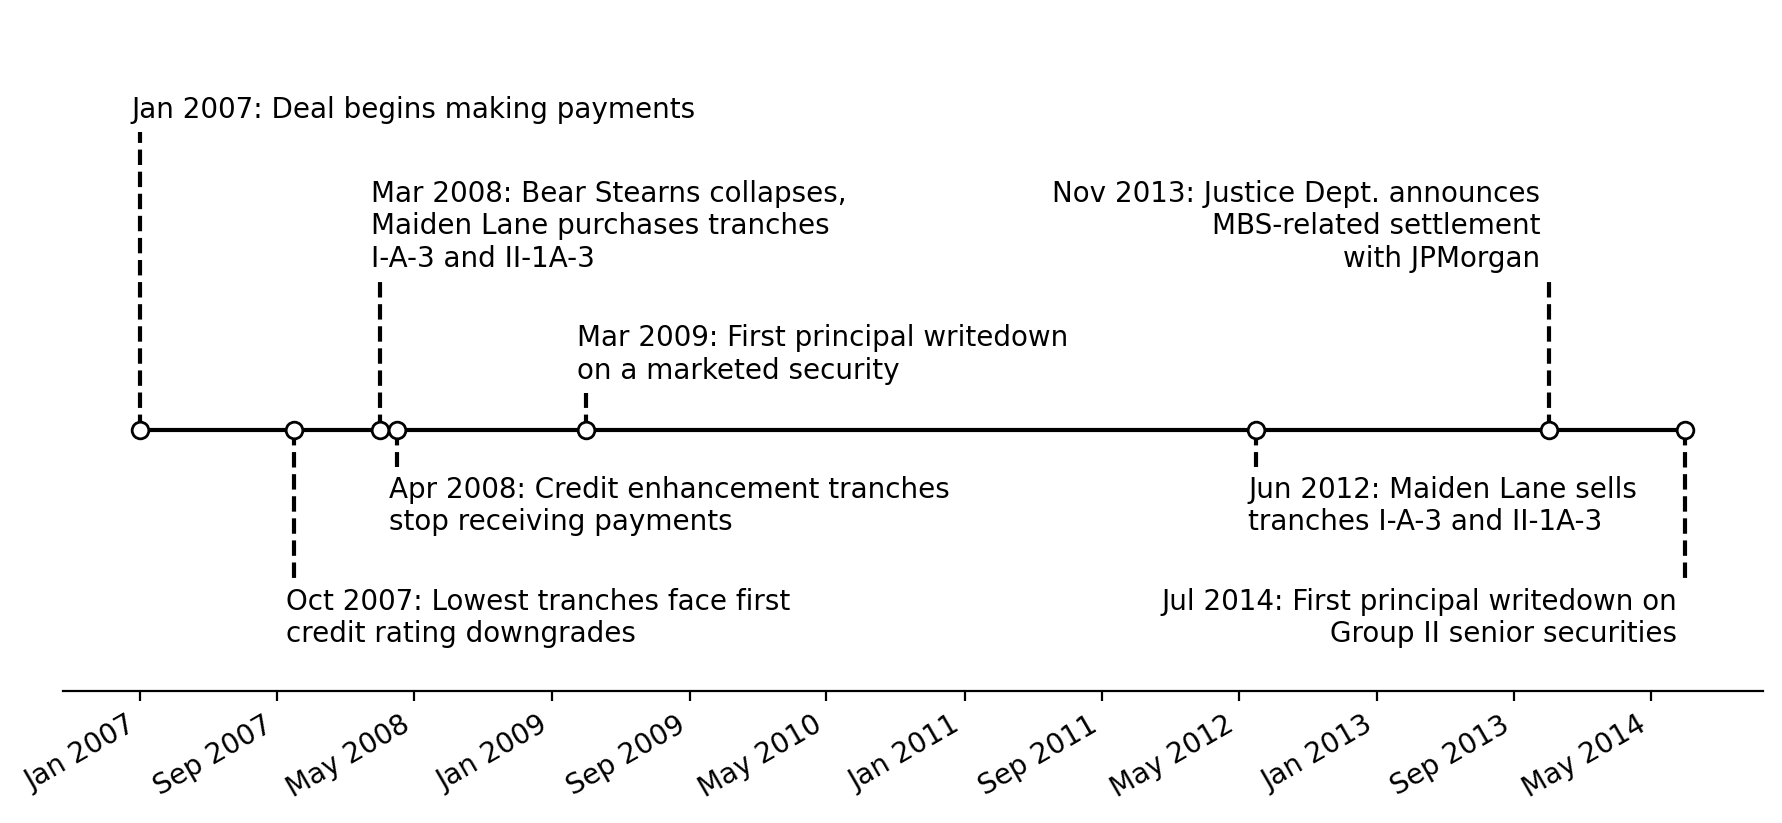
\includegraphics[width=0.8\textwidth]{../figures/timeline_of_important_events}
	\label{fig:timeline_of_important_events}
\end{figure}

\subsection*{Overall Levels of Writedowns}

Now, over a decade after their initial issuance, we’ll begin our analysis by getting a high-level picture of how much each security has suffered in principal writedowns. In Group I, all of the mezzanine securities from I-M-3 through I-M-9 had 100\% of their principal written off due to poor performance by the mortgage pool, tranche I-M-2 has had approximately 78\% of its principal written off, and tranche I-M-1 has emerged from the financial crisis unscathed, taking no writedowns, but not receiving any principal payments either. In Group I, realized losses made impacts even higher up the subordination totem pole, with every single mezzanine tranche being completely wiped out, leading to each of the Group II senior tranches starting to take losses which are allocated pro rata within that collection of securities. Overall, mezzanine securities have had 91\% of their principal written off, while senior securities across the two groups have lost only about 5\% of their original face value through writedowns. Of an original total marketed certificate balance of \$1.09 billion, only \$182 million is still outstanding, and \$258 million of the certificate holders’ original investment has been lost due to defaults among the deal’s underlying mortgages, for a loss rate of 23.5\%, a figure that would surely make most investors cringe. So, in a vacuum, before considering the actual principal and interest payments that have been made to these securities throughout their lives, we can say that 23\% of the original face-value principal balance in this deal will never be paid back to investors. Of course, because of the fundamental credit-enhancement systems built into an MBS deal, these losses are allocated far from evenly, so understanding how any individual security performed takes a bit more work.

To get a rough estimate of the degree of credit protection experienced by a particular security at any point in time, we can use a graph which represents balances of securities in each group as percentages of the total remaining principal in their respective groups. So, everything below a particular security’s band on the graph is “protecting” it, in the sense that mortgage losses equal to the total remaining balance on ALL of the more subordinated securities would have to occur before the one in question would suffer any writedowns. One other helpful feature of this type of graph is that it allows us to distinguish between principal payments and writedowns in terms how they affect the deal’s overall principal balance. Securities that have their principal balances fully paid off by remittances from mortgage borrowers slowly disappear at the top of the graph, and securities which are fully written off - due to the servicer confirming losses on mortgages - disappear at the bottom of the graph.


\begin{figure}[h]
	\centering
	\caption{Subordination Levels in Group I}
	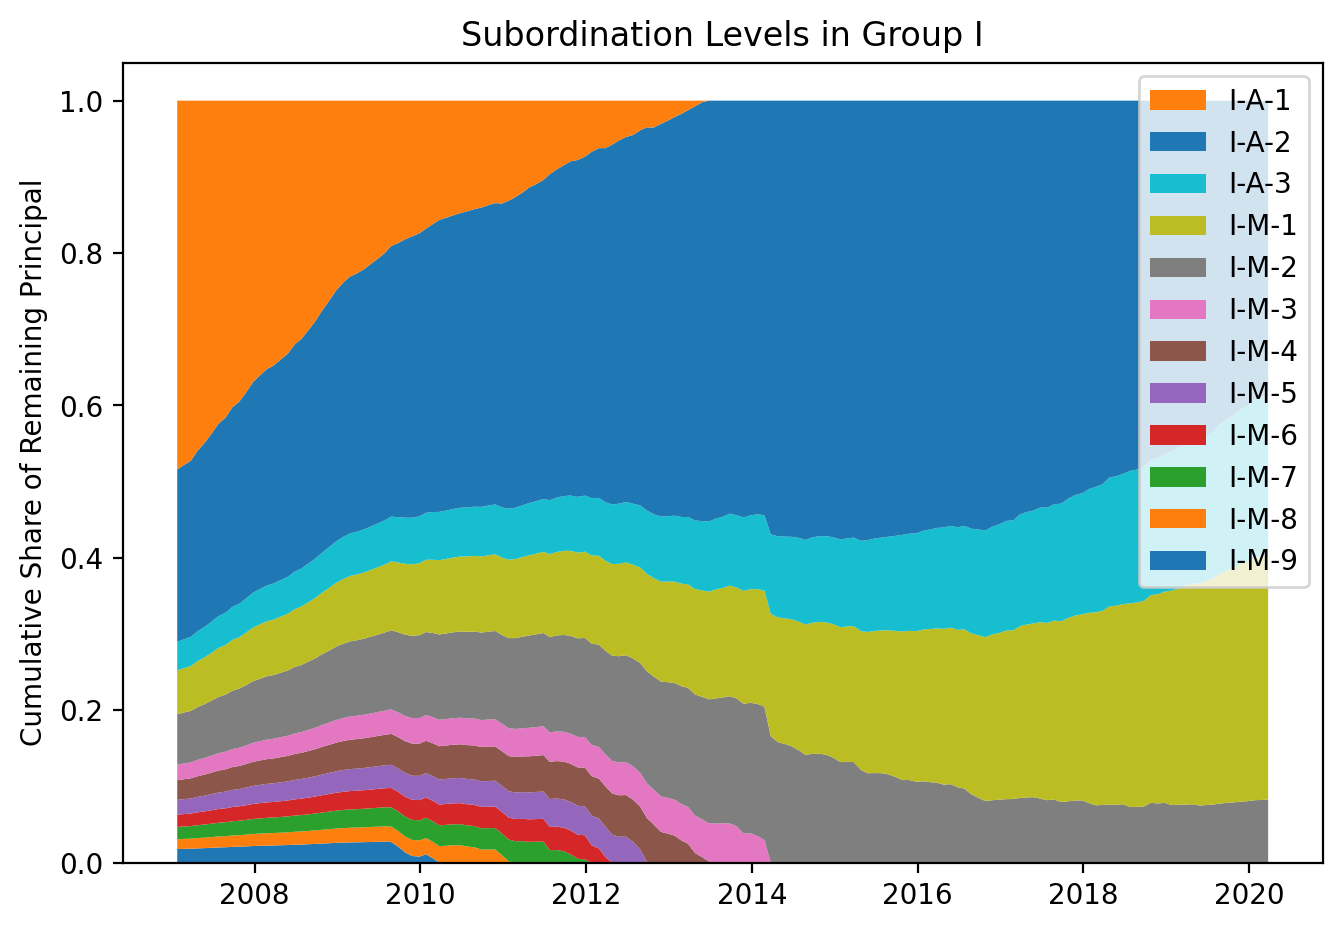
\includegraphics[width=0.8\textwidth]{../figures/stackplot_share_of_principal_group_i}
	\label{fig:stackplot_share_of_principal_group_i}
\end{figure}

\begin{figure}[h]
	\centering
	\caption{Subordination Levels in Group II}
	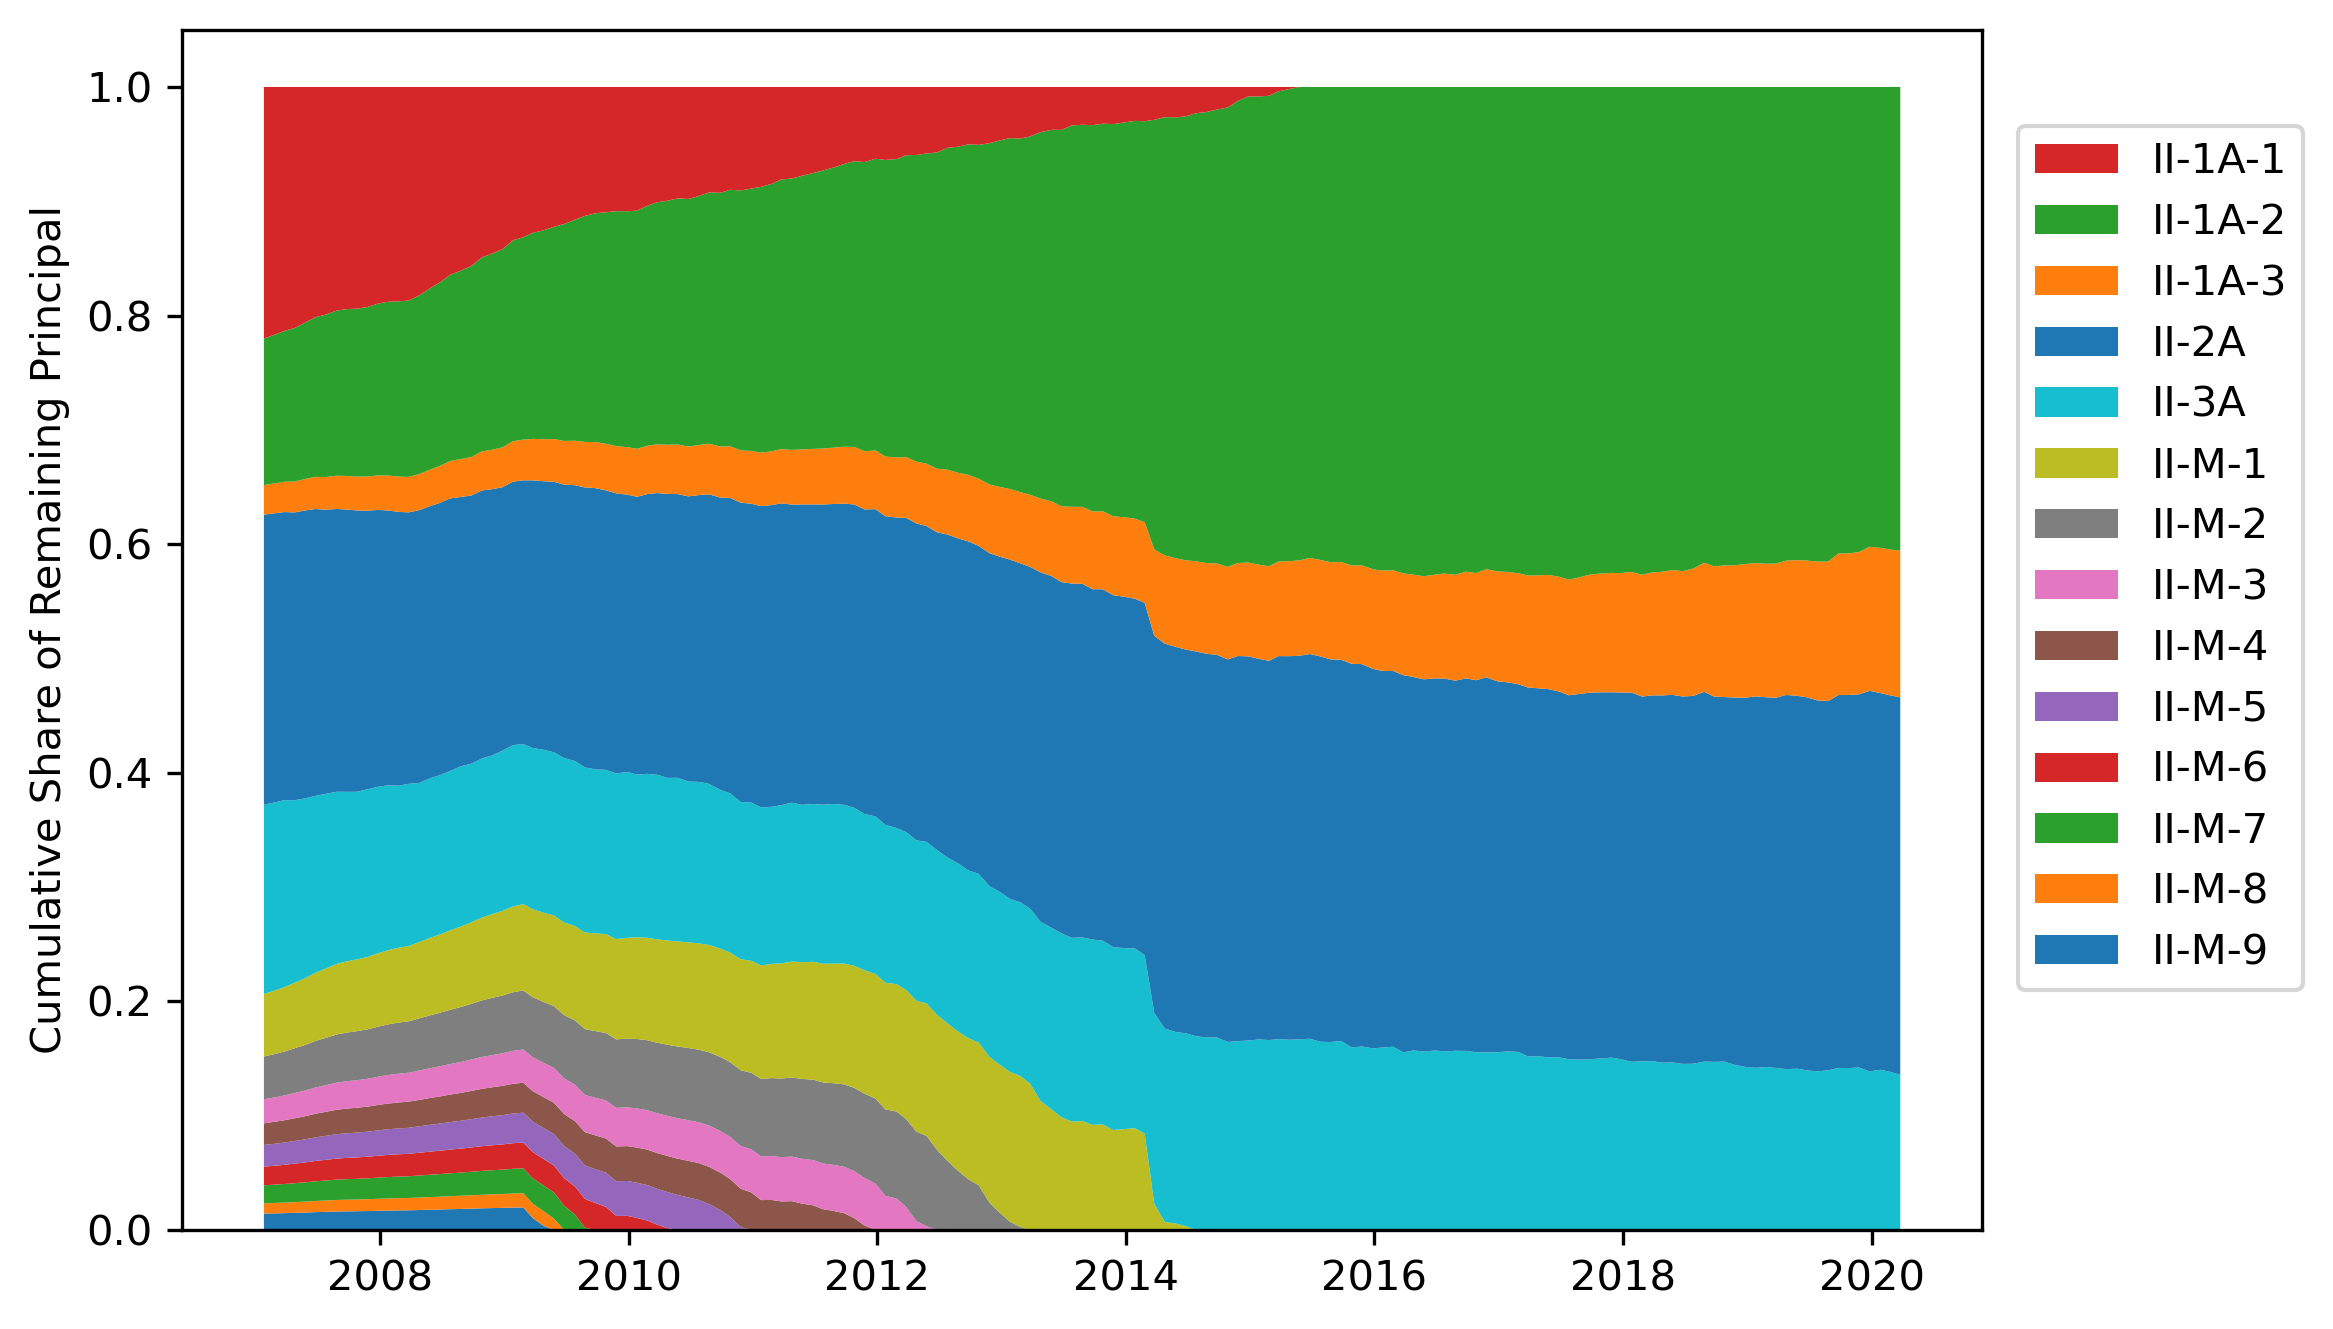
\includegraphics[width=0.8\textwidth]{../figures/stackplot_share_of_principal_group_ii}
	\label{fig:stackplot_share_of_principal_group_ii}
\end{figure}

This figure provides a useful comparison for understanding how confident a holder of a senior-level security can feel about eventually getting their money back. In Group I, at least 20\% of the remaining principal balance is always taken up by mezzanine securities, so at any point so far, senior-level investors have known that over 20\% of the remaining security principal would have to be written off before they would be hurt at all. However, in Group II, by mid-2014, the senior securities were directly exposed to any future realized losses on the mortgages, since the buffer provided by the existence of mezzanine securities had completely evaporated. These figures also illustrate a point about the composition of mortgage-backed securities that perhaps goes unnoticed by many. Despite the popularity of stories of daring hedge fund managers like Michael Burry winning big by betting against risky mezzanine tranches, the majority of the principal is concentrated in the senior securities, which offer relatively low interest rates and will take many years to be fully paid off.


\subsection*{Importance of ``Lower Senior'' Tranches}

The subordination-levels graphs also illustrate one way in which I interpret the desirability of each kind of security in this deal, and in MBS deals in general. The highest-level senior securities (like I-A-1 in Group 1) have very low interest rates, but are also low-risk and are likely to be paid off first, making them a great choice for institutions that need to park their cash somewhere with a secure, positive return. The mezzanine tranches are significantly higher-risk, but they present much more attractive interest rates, for the exact reasons that this deal demonstrates – they will likely be the last to receive principal payments, and they do not enjoy the benefits of subordination to the extent that senior securities do. This leaves the “lower senior” securities, like I-A-3 in Group I and II-3A in Group II, in an odd state of limbo. Because they are still senior-quality and are unlikely to suffer significant losses, they don’t offer very attractive interest rates, and yet they are also likely to be the last securities still standing in the deal. As we can see in Figure 2, these lower senior tranches make up the majority of the principal balances remaining in both groups at the moment, since the highest-ranked senior securities (at least in Group I) have been fully paid off, while the mezzanine securities have been mostly wiped out by losses. Due to the mortgages’ overall poor performance, the lower senior securities are still receiving only meager principal and interest payments, so investors in these particular tranches will likely have their money tied up in this deal for quite a while. In my opinion, this makes these securities somewhat less desirable in comparison to the higher senior securities and the mezzanine ones, as “lower senior” status offer neither the near-absolute insulation from principal losses of a I-A-1 nor the chance at excellent yields offered by those such as a I-M-7 or a I-M-9. So, beyond the simple ordering of securities presented by a deal’s prospectus, in which each tranche is simply less risky than all those below it, breaking down these securities into three general categories may be a helpful tool for understanding deals like this one from the perspective of investors. Despite the fact that all of the securities in Group I are based on the same underlying mortgage pool (and likewise for Group II with its own mortgage pool), the previous figure reminds us that investors should have significantly different expectations for how their money will perform depending on where they choose to locate themselves within this hierarchy of securities.


\section*{Part III: The Mortgages}
\subsection*{Summary of Cash Flows}

Now that we have summarized essential features of this deal’s origination and history, we will attempt to build a bottom-up understanding of its performance since 2007 by examining its mortgage pool in greater detail. From here on, even though this deal’s securities are technically based on two separate groups of mortgages, Group I and Group II, the two groups will be referred to jointly when discussing their performance. On the next page is some useful basic information about the mortgages’ performance:

\begin{table}[h]
	\centering
	\begin{tabular}{| l  | l  |}
\hline
Mortgage pool size in January 2007 & \$1.143 billion \\
Mortgage pool size in March 2020 & \$183 million \\
Total prepayments on mortgages & \$294 million \\
Total principal remitted to the MBS trust & \$461 million \\
Total realized losses on the mortgage pool & \$510 million \\
Mortgage loss rate (realized losses divided by original pool size) & 44.6\% \\
\hline
\end{tabular}
	\caption{Mortgage Performance Summary}
	\label{tab:table_deal_summary}
\end{table}

Even just this high-level information is enough for us to begin to tell a story about these mortgages’ performance. Right off the bat, we notice that realized losses on this group of mortgages, which covered wide ranges of borrower creditworthiness, principal size, and geographic location, were over 40\% of the initial principal balance, a figure that would cause any sensible investor to shudder. This alone makes it clear that the quality of these mortgages was shaky at best. Of course, countless pages have already been written regarding to what extent we could have known this about subprime mortgages before the financial crisis of 2007, so we will not go into much depth about that topic here. Next, we observe that cumulative realized losses have exceeded the total principal payments distributed to investors since January 2007, bringing us to the remarkable conclusion that of all the mortgage principal that has dropped out of the deal since its inception, roughly half has been “bad” rather than “good”. The following graph gives us more useful information about the evolution of the mortgage principal pool over time:

\begin{figure}[h]
	\centering
	\caption{Distribution of Loan Statuses for Remaining Loans}
	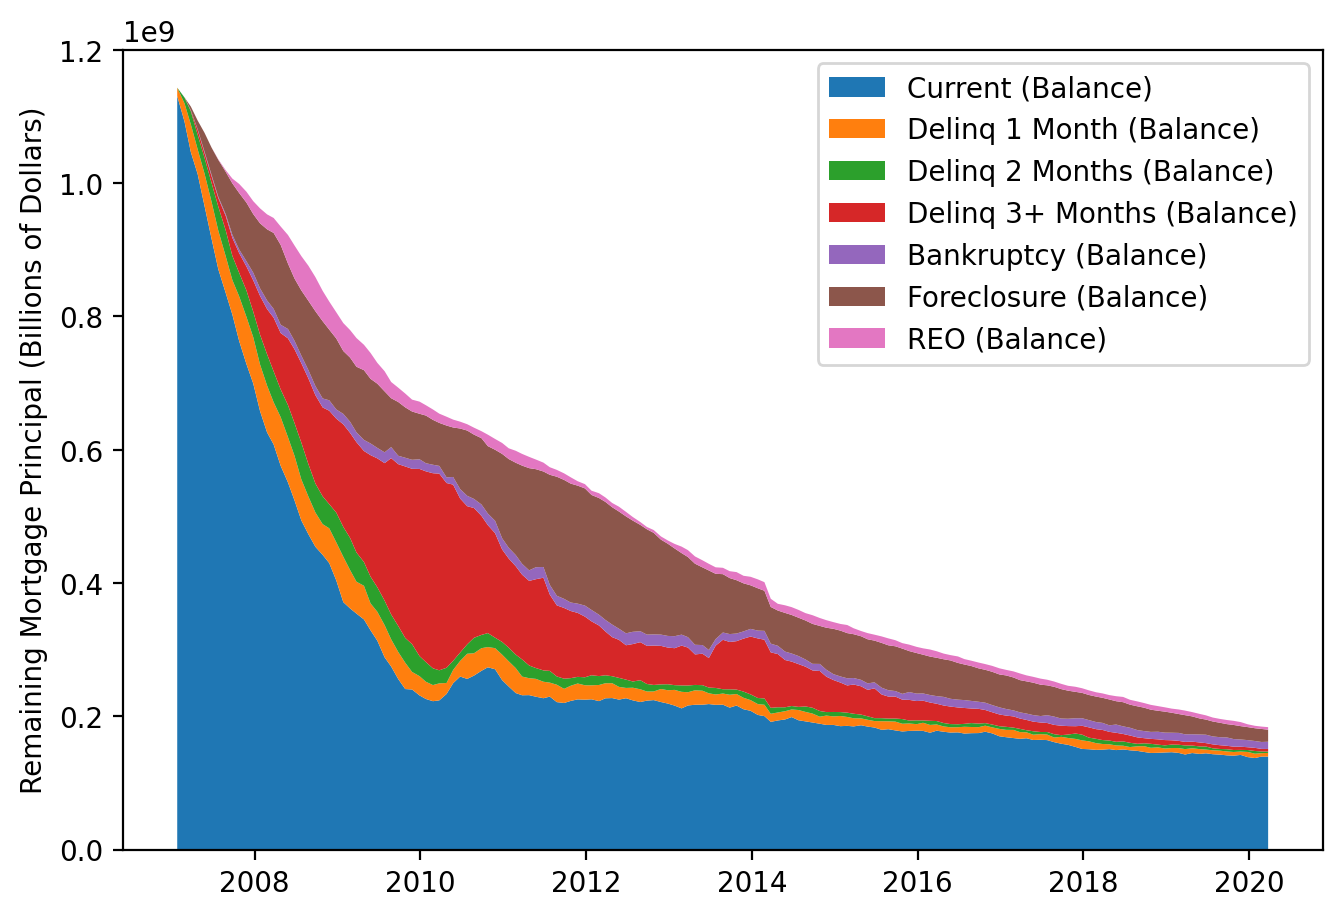
\includegraphics[width=0.8\textwidth]{../figures/stackplot_delinq_status}
	\label{fig:stackplot_delinq_status}
\end{figure}

We can see here that the shock to housing markets in the wake of the Great Recession had effects on this deal until 2014 or so, much longer than one might expect. Specifically, as the Great Recession reached its peak, there was a major uptick in the total value of loans for which borrowers were at least 3 months delinquent, and it took until around mid-2010 for this to fall back down. Of course, delinquency is only the beginning of the story: the loans that are severely delinquent move through the bankruptcy process, then they end up in foreclosure, where Bear Stearns will try to recoup as much of its losses as possible by selling off the borrower’s house. Looking at only the total loan balances held by delinquent borrowers would suggest that the detrimental effects of the Great Recession had mostly worn off by 2011 or so, but when we also consider the way in which the number of loans undergoing foreclosure jumped after the spike in delinquencies, we get a more complete picture of how the housing market was significantly shaken by the events of 2007-08. The foreclosure process is the last major part of the mortgage life cycle for this deal, and we see above that it took until 2014 for the glut of foreclosed-upon loans in this deal to mostly dissipate. A large number of loans in foreclosure makes it even tougher for investors to judge how much of their principal they’ll be getting back, since while a loan is delinquent, the mortgage servicer can try its best to negotiate modified payment plans with borrowers, but once the underlying home is foreclosed on, investors become exposed to the demand for foreclosed-upon homes, not just the financials of the original borrowers.

	As the total remaining mortgage principal balance shrinks, the rest has to go somewhere, and we can sort all of the disappearing principal into two buckets: “remittances to trust” – including prepayments and regularly scheduled payments – and “written off” (investors receive the former, and the latter is defaulted-on principal that cannot be recovered). By adding these series to the previous graph, we can further improve our understanding of where all the mortgage principal is going.


\begin{figure}[h]
	\centering
	\caption{Distribution of Loan Statuses, Including Payments, Prepayments, and Writedowns}
	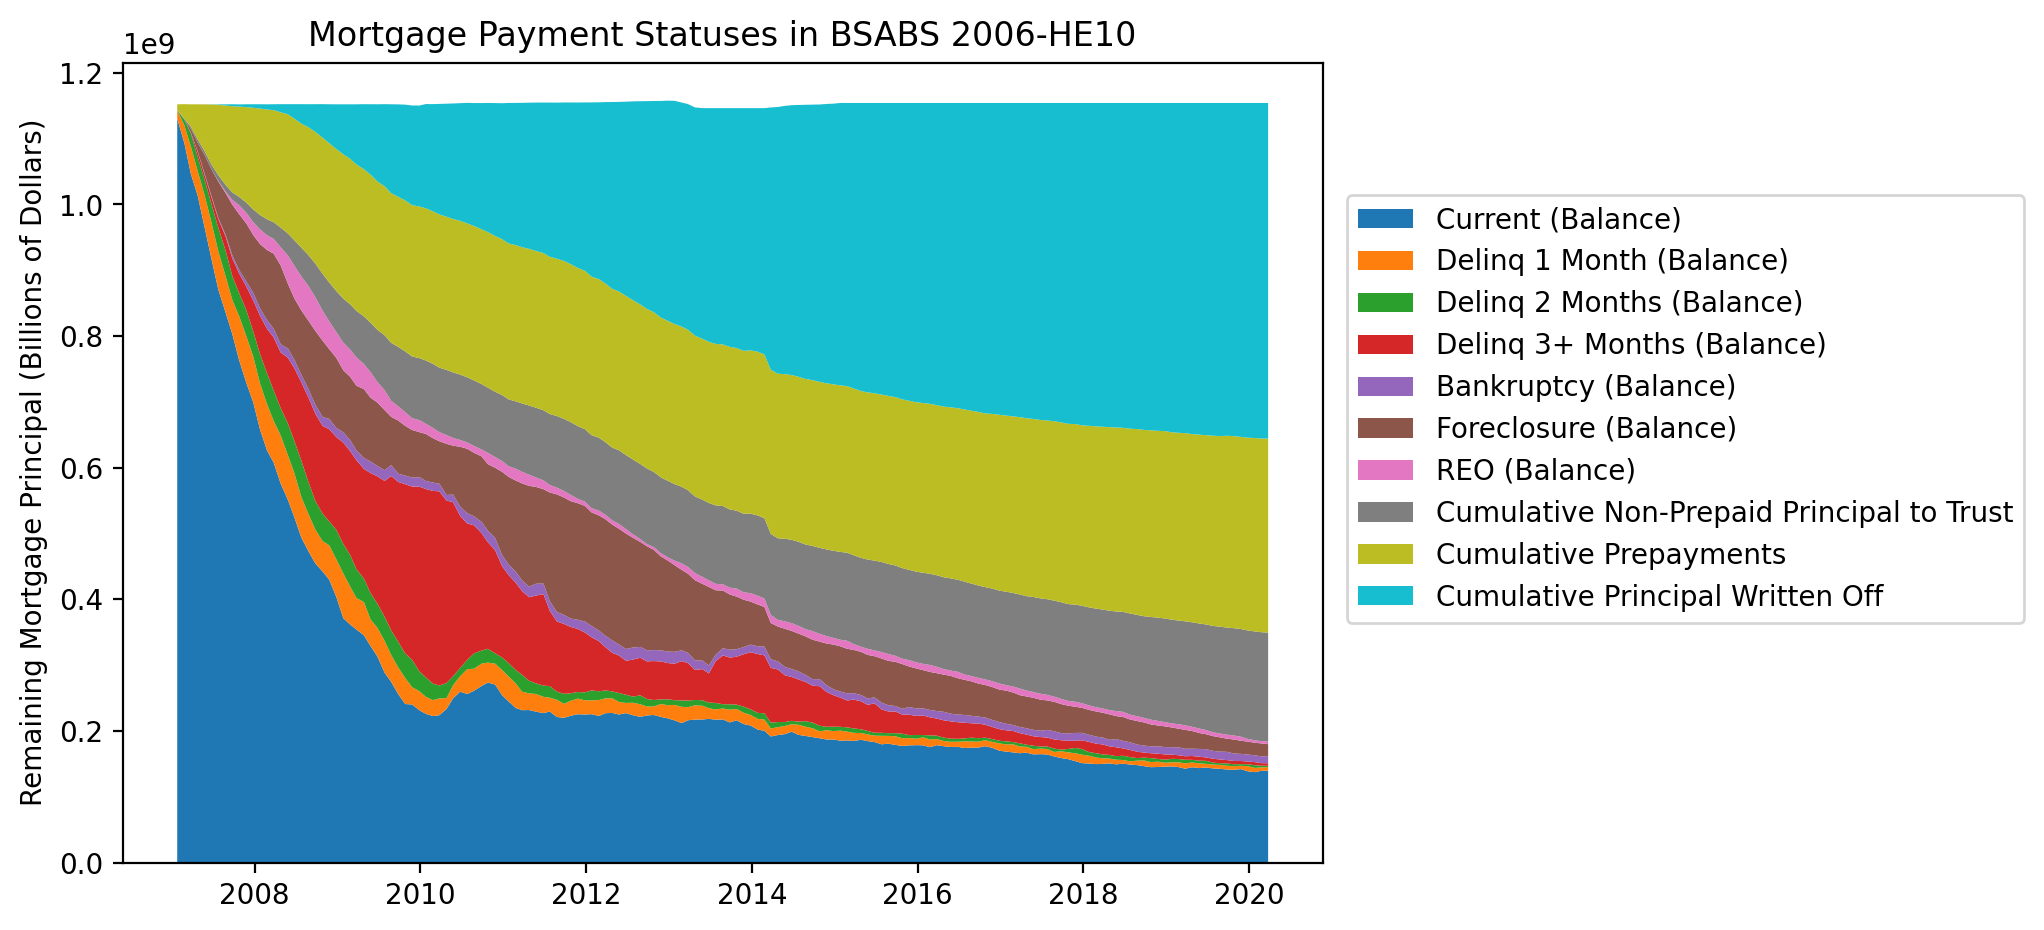
\includegraphics[width=0.8\textwidth]{../figures/stackplot_delinq_status_with_writeoffs}
	\label{fig:stackplot_delinq_status_with_writeoffs}
\end{figure}

Although these columns do not perfectly add up to the original principal balance of \$1.143 billion, their sum is remarkably close to that figure across the deal’s life, signaling that we’ve managed to almost completely account for the flow of principal out of the deal. The “Cumulative Non-Prepaid Principal to Trust” segment is calculated as total principal remitted to the trust minus total mortgage prepayments, the “Cumulative Prepayments” segment is the total value of prepayments by borrowers, and the “Cumulative Principal Written Off” segment is the sum of all realized losses on the mortgage pool over time. For an investor, it would be quite disconcerting to see that over \$500 million of the original principal balance in the mortgage pool has been written off due to defaults (as of March 2020), while slightly less than that has actually been paid out to security holders after 12 full years of mortgage payments. We will examine in greater detail how investors were affected by these losses in Part IV.


\subsection*{Understanding the Deal's Prepayment Patterns}

In addition to the realized losses that are so important for determining the value of investors’ MBS holdings, prepayments introduce an extra layer of uncertainty, and the evolution of the prepayments for this deal’s mortgages gives us another perspective on how the financial crisis profoundly affected mortgage borrowers. Prepayments through March 2020 totaled almost \$300 million, larger than the sum of regularly scheduled principal payments, but they were also very unevenly distributed through time, as shown below:

\begin{figure}[h]
	\centering
	\caption{Time Series of Mortgage Prepayments}
	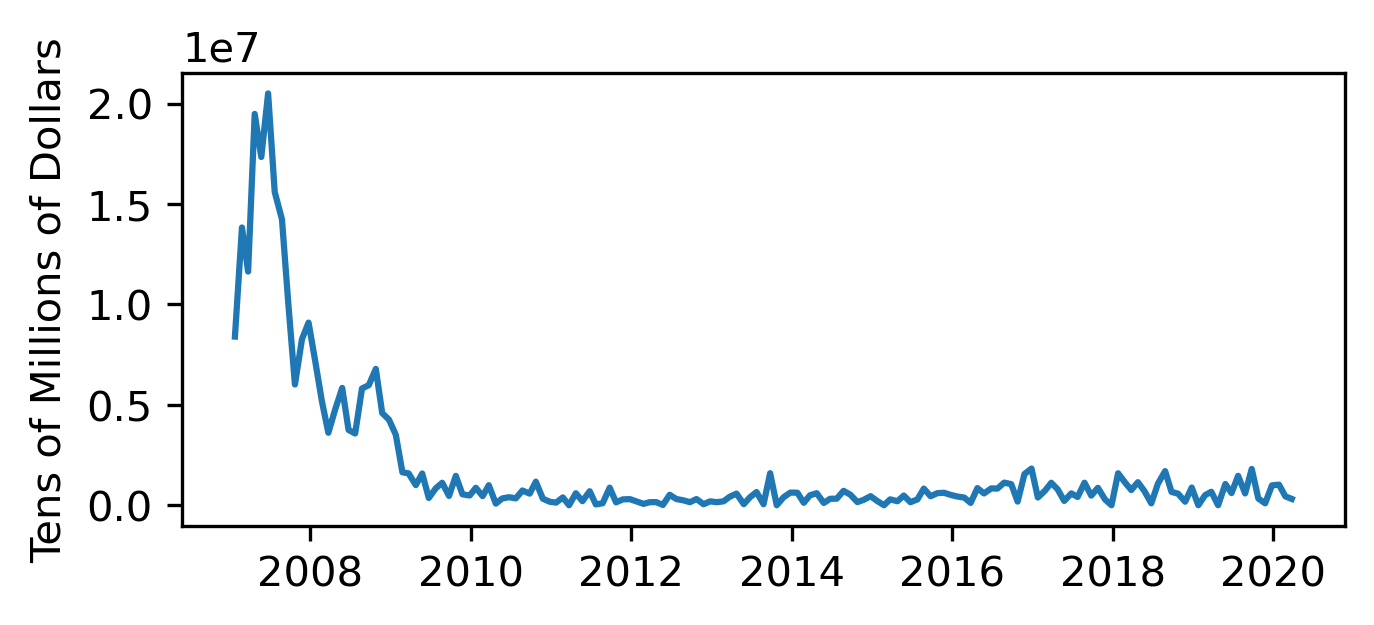
\includegraphics[width=0.8\textwidth]{../figures/timeseries_prepayments}
	\label{fig:timeseries_prepayments}
\end{figure}

In normal times, a high level of prepayments can spark enthusiasm for investors in mezzanine tranches, as it can be a strong indicator that a “stepdown” is coming. This means that the deal is performing so well that instead of making principal payments to the most senior tranche first, which is the usual structure, the cash flow hierarchy will change so that the lowest tranche will get principal payments each month instead. This practice of trying to pay off the lowest-rated securities first has the potential to save a lot of money for the issuer: the lowest tranches pay out the highest interest rates of any securities in the deal, and in some MBS designs, the issuer will get to pocket any extra interest that’s left over after making all required payments to the remaining securities. If this stepdown occurs, speculators in high-risk tranches will have reason to become much more confident in their future returns. On the opposite end of the spectrum, though, a trend of increasing delinquencies and foreclosures rather than prepayments would spell danger even for securities with substantial credit enhancement, and the rapid decline in prepayments that we observe in Figure 5 seems to reflect a drastic change in borrowers’ behavior.

	Based on Figures 3-5, we can dig a little deeper into how the composition of the deal’s loan pool changed over time. Our starting point for this will be a review article on the subject of MBS prepayment risk by Sean Becketti, an economist at the Kansas City Fed, which lists three main events that can trigger rapid changes in a mortgage’s principal balance: refinancing, relocation, and default. In his summary, Becketti points out that the most important driver of refinancing is the relative gap in interest rates between a borrower’s current mortgage and others available on the market, while relocation is more intuitively driven by borrowers’ major life events (like changing jobs or getting married), and default is strongly related to overall macroeconomic conditions. Using data on government-backed Fannie Mae MBS, Becketti reached the conclusion that mortgage borrowers’ behavior follows a clear pattern: prepayments are low at first, then they peak three or four years after origination due to relocations and the desire to refinance, and then they settle down to a stable long-term level after that.
	
If this really is the standard pattern of prepayments, then BSABS 2006-HE10 defies the usual trends seen in MBS loan pools, as it had tens of millions of dollars in prepayments within its first 1.5 years of existence, but then prepayments dropped to near-zero levels as the Great Recession took hold. Since interest rates were slashed by the Fed in response to the 2007 financial crisis, we would naively expect a rise in prepayments as financially savvy borrowers noticed that they could switch to a much cheaper mortgage. However, in this case, it appears that any appeal of refinancing was overwhelmed by the economic distress that the deal’s borrowers felt due to the national recession. So, when such a massive macroeconomic shock occurs, it seems to become more difficult to differentiate between forces driving prepayments and forces driving defaults. If there really were a large number of borrowers in this deal who were financially comfortable and rationally examined interest rate patterns to decide when to refinance, then we might have seen a more standard prepayment time path, where prepayment rates rise for three or four years until the deal is “seasoned” (the industry term for a deal whose prepayment risk has reached a stable level). Instead, while there was a slight rebound in prepayments in 2008 as the Fed cut rates, delinquencies spiked on a national scale while prepayments mostly plummeted, suggesting that general macroeconomic conditions were a much more immediate concern for borrowers than the option to shave a few basis points off their mortgage rates by putting time and money into refinancing. For many borrowers, a significant drop in their home’s value was likely much more salient than falling interest rates, and in some situations, the potential benefits of simply defaulting on a “underwater” mortgage – meaning that the outstanding principal balance is higher than the value of the home – may have been more appealing than attempting to capture some marginal savings by refinancing at a lower rate.

In the big picture, both prepayments and delinquencies reached very low levels by the second half of the 2010s, telling us that the deal’s payment patterns have stabilized, and that most borrowers at this point are making their payments each month but not doing anything else too exciting. So, the deal would definitely be referred to as “fully seasoned” by now, but its first few years after origination definitely showed out-of-the-ordinary prepayment and default behavior. Although experts did acknowledge that MBS deals exhibit “considerable idiosyncratic prepayment risk” \textcite{becketti89} decades ago, there is still much more to be done in terms of understanding how both financial and macroeconomic factors influence a single borrower’s preferences – they’re always thinking about refinancing, defaulting, relocating, or doing none of the above – rather than considering each of these possible behaviors in isolation.


\subsection*{Fixed vs. Adjustable-Rate Loans}

One other useful angle from which to analyze the composition of this deal’s mortgage pool is by breaking it down into fixed- and adjustable-rate loans. A major part of the public narrative about the collapse of the housing market in 2007 was the prevalence of adjustable-rate loans issued with weak underwriting standards to households with lackluster credit scores, so it makes sense to take a look at how risky this deal’s ARM loans actually turned out to be, compared to their fixed-rate counterparts.

At the deal’s inception in early 2007, adjustable-rate loans made up roughly 76\% of BSABS 2006-HE10’s mortgage pool (with fixed-rate as the remaining 24\%), matching up with the common perception that banks specifically chose to focus on originating adjustable-rate loans – which would potentially offer higher returns for investors if global rates like LIBOR remained high – in order to securitize them. At this point, it should be mentioned that this “baseline” composition of the pool here is actually from the March 2007 data, not when reports were first issued in January 2007, since the number of loans in the deal doesn’t actually peak until March; my best guess as to why this occurs is that the loans in the deal were all originated in 2006, but it took until March of 2007 to finish packaging all of them into this securitization. With that in mind, the first plot of interest when comparing fixed vs. ARM loans is a comparison of overall delinquency rates between the two groups:


\begin{figure}[h]
	\centering
	\caption{Delinquency Rates for Fixed- and Adjustable-Rate Mortgages}
	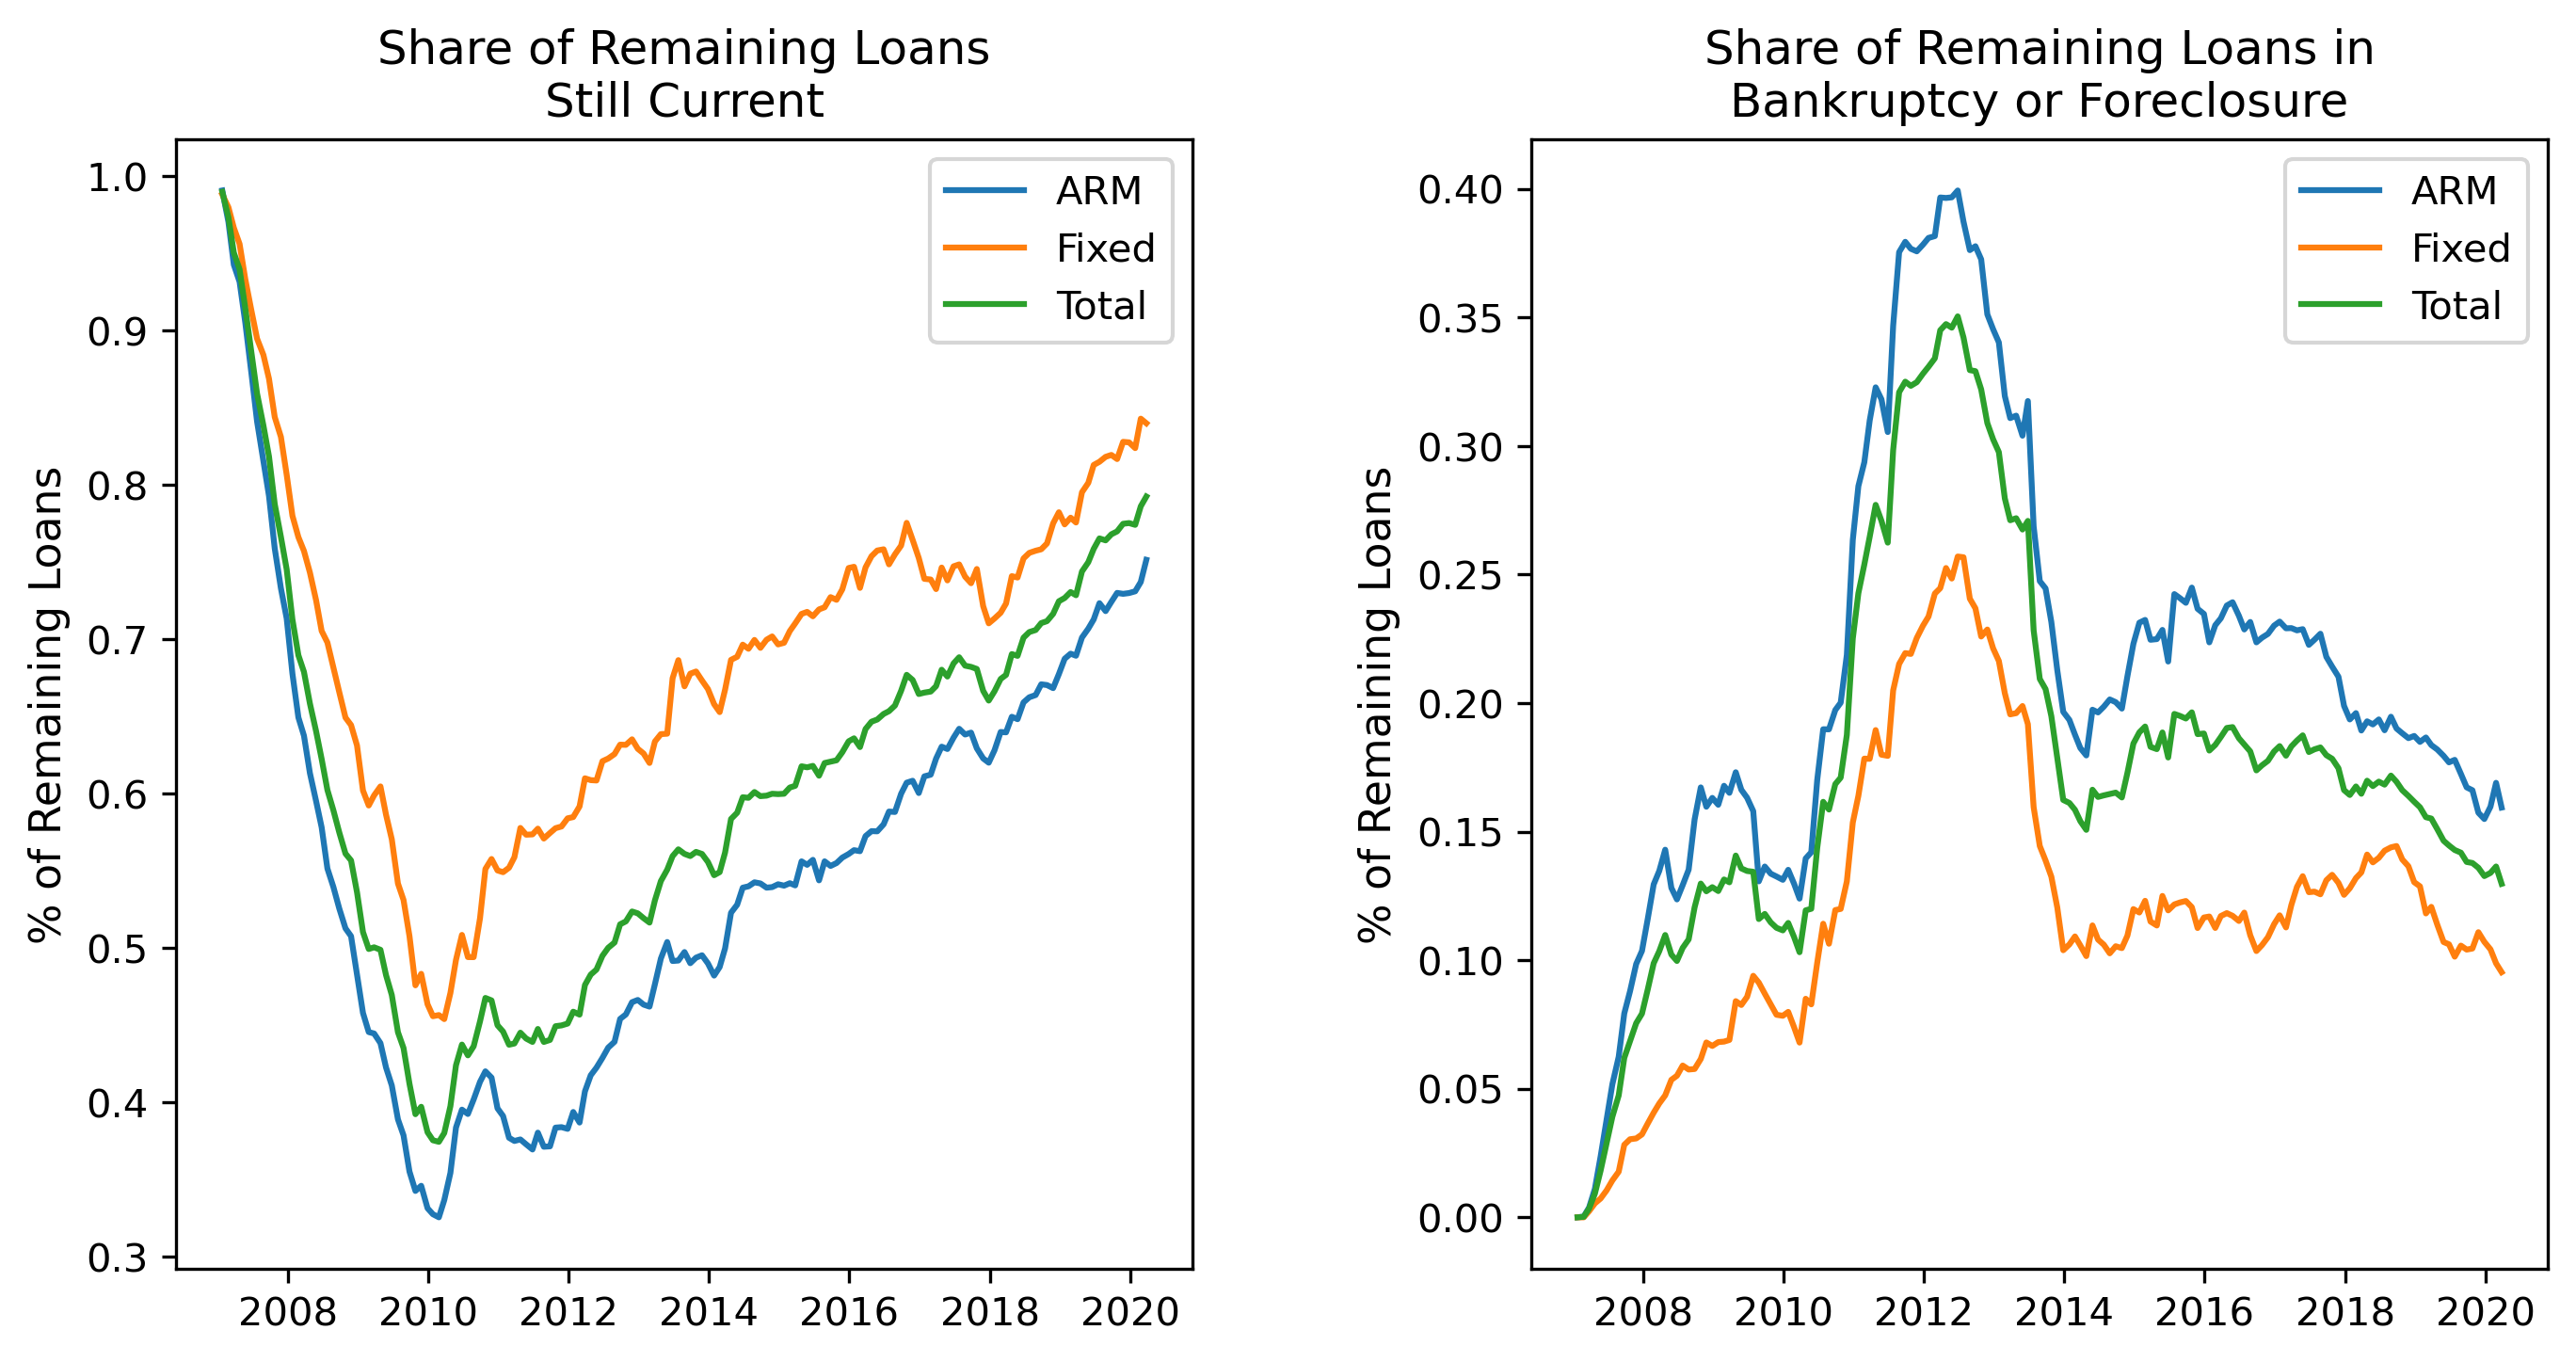
\includegraphics[width=0.8\textwidth]{../figures/timeseries_delinq_status_fixed_vs_arm}
	\label{fig:timeseries_delinq_stats_fixed_vs_arm}
\end{figure}

The left plot displays the portion of the remaining outstanding loan balance at any point in time for which borrowers were still up to date on their payments. For example, it shows that out of all ARM borrowers whose loans were still outstanding in early 2010, less than 35\% of them were still staying current on their mortgage payments. The right-side plot shows the population of the other end of the delinquency spectrum, specifically what percentage of the remaining loan balance was in either bankruptcy or foreclosure, which is relevant because these two statuses are what imply that a borrower is all but done for, and that the mortgage servicer is going to have to liquidate the associated house for whatever they can get. Taken together, these two plots make it clear that borrowers with adjustable-rate loans were hit harder by the Great Recession than their fixed-rate counterparts, as ARM borrowers were more likely to enter bankruptcy and less likely to stay current on payments than their fixed-rate counterparts. In order to see how this differential might translate through to losses on investors’ securities, the next step is to check on what the cumulative “loss rates” were, i.e., what percentage of the original principal balance had been written off as realized losses after the bankruptcy/foreclosure process was complete. Unfortunately, due to a change in trustee for this deal in 2013, the investor reports after May of that year do not break out the monthly realized loss figures into adjustable- and fixed-rate segments, so the best we can do is to use the cumulative broken-out realized loss numbers from the original trustee, which means we can only evaluate this component of the deal up through mid-2013. This summary information for the aggregated fixed- and adjustable-rate loan groups is displayed here, with an expanded version of the table which breaks out every single type of loan present in this deal available in Appendix B:


\begin{table}[h]
	\centering
	\begin{tabular}{| l | l | l |}
\hline
  & \textbf{ARM} & \textbf{Fixed} \\
\hline
Number of Loans (March 2007) & 3,405 & 1,668 \\
Principal Balance (March 2007) & \$847 million & \$268 million \\
Loss Rate (baseline is March 2007) & 32.0\% & 30.0\% \\
Share of Initial Principal & 76.0\% & 24.0\% \\
Share of Realized Losses Through May 2013 & 77.3\% & 22.7\% \\
\hline
\end{tabular}
	\caption{Realized Losses by Mortgage Type (through May 2013)}
	\label{tab:table_realized_losses_fixed_vs_arm}
\end{table}

The following graph gives some extra context to these figures by plotting the cumulative loss rate (the third column in the table) over time:

\begin{figure}[h]
	\centering
	\caption{Cumulative Principal Losses for Fixed- and Adjustable-Rate Mortgages}
	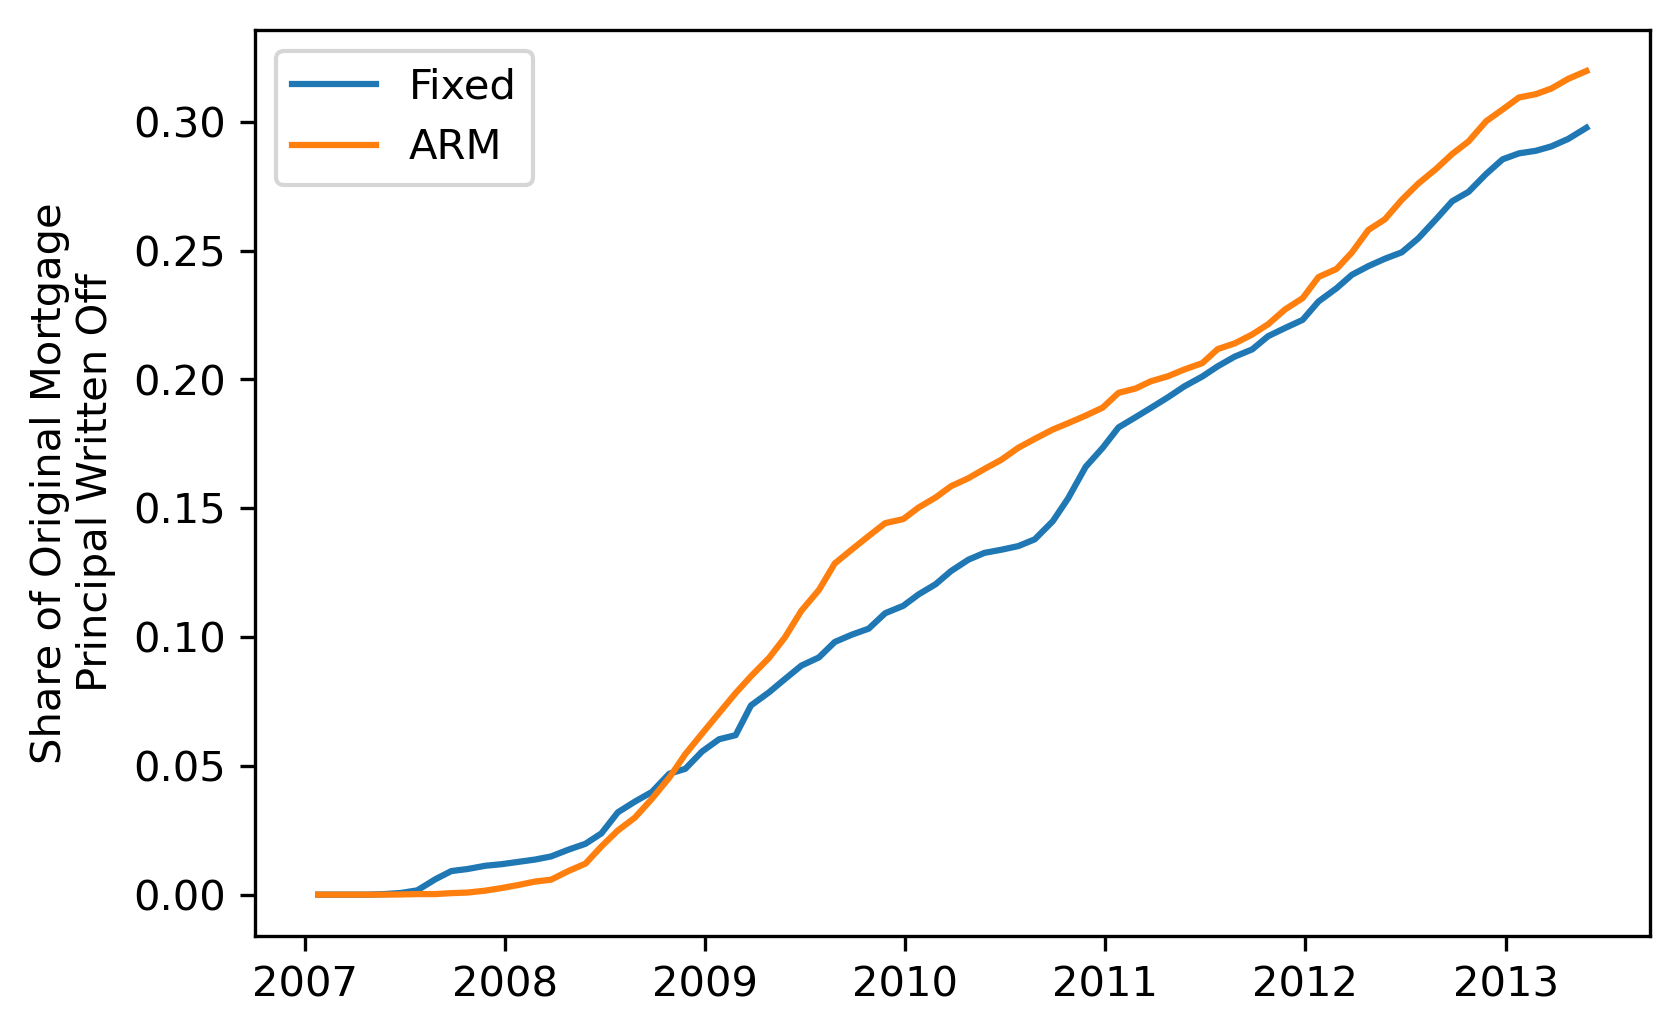
\includegraphics[width=0.8\textwidth]{../figures/timeseries_cumulative_losses_fixed_vs_arm}
	\label{fig:timeseries_cumulative_losses_fixed_vs_arm}
\end{figure}

So, contrary to what the previous graphs suggested about ARM loans performing much worse than fixed-rate loans, the data up through May 2013, a few years after the recession officially ended, actually suggest that adjustable-rate loans were not all that much more toxic than fixed-rate loans – by May 2013, adjustable-rate mortgages had had 32\% of their March 2007 principal balance wiped out through write-offs, while the corresponding figure was 30\% for fixed-rate mortgages. Does this mean that ARM loans are actually no riskier for investors, and that MBS speculators should only invest in deals that are filled to the brim with adjustable-rate mortgages? Well, not quite. Because we’re unable to break down the mortgage loss numbers by fixed- vs. adjustable-rate after 2013, my preferred explanation for why the stories told by Figure 6 and Table II are so different is that not all of the realized losses which resulted from the delinquencies shown in Figure 6 were actually finalized and booked by May 2013. As far as I can tell after reading through this deal’s documentation, realized losses on each delinquent loan are only recorded after a loan has completed the foreclosure process and the servicer has liquidated the house for as much as they can get. So, because Figure 4 tells us that there were still a significant number of loans in the foreclosure stage in May 2013, it could be the case that even though realized losses on those loans were in fact disproportionately weighted towards ARMs, we just can’t see that because the associated losses were not recorded until after May 2013.

In summary, the data available for this deal do suggest that adjustable-rate loans performed somewhat worse than their fixed-rate counterparts in terms of borrowers staying current and avoiding default, but we are unable to fully quantify how this disparity affected MBS investors due to limitations with the mortgage principal loss series in the investor reports. Now that we’ve gotten a better feel for how the underlying mortgages in this deal performed, the time has come to circle back to the securities that are the true focus of our analysis and hunt for some more answers about just how toxic they turned out to be.


\section*{Part IV: Consequences for MBS Investors}

\subsection*{Where Are the Securities' Principal Payments Coming From?}

The fundamental appeal of an MBS, or any similar type of asset-backed security, is that the security’s complex structure softens the blow felt by investors when the underlying asset becomes delinquent or gets marked down somehow, so the big question that we need to answer is just how much benefit that complex structure provided. We know that BSABS 2006-HE10 had excess spread and overcollateralization mechanisms in place, so the true test of the value of this securitization structure is the extent to which it could protect investors during the worst housing market crash in decades. Part of this question is just about determining what fraction of losses on mortgages ended up affecting the overall group of security holders, but it’s also important to know how holders of different tranches were affected. The starting point for this analysis is the following figure: 

\begin{figure}[h]
	\centering
	\caption{Principal Writedowns on Mortgage Pool and Securities}
	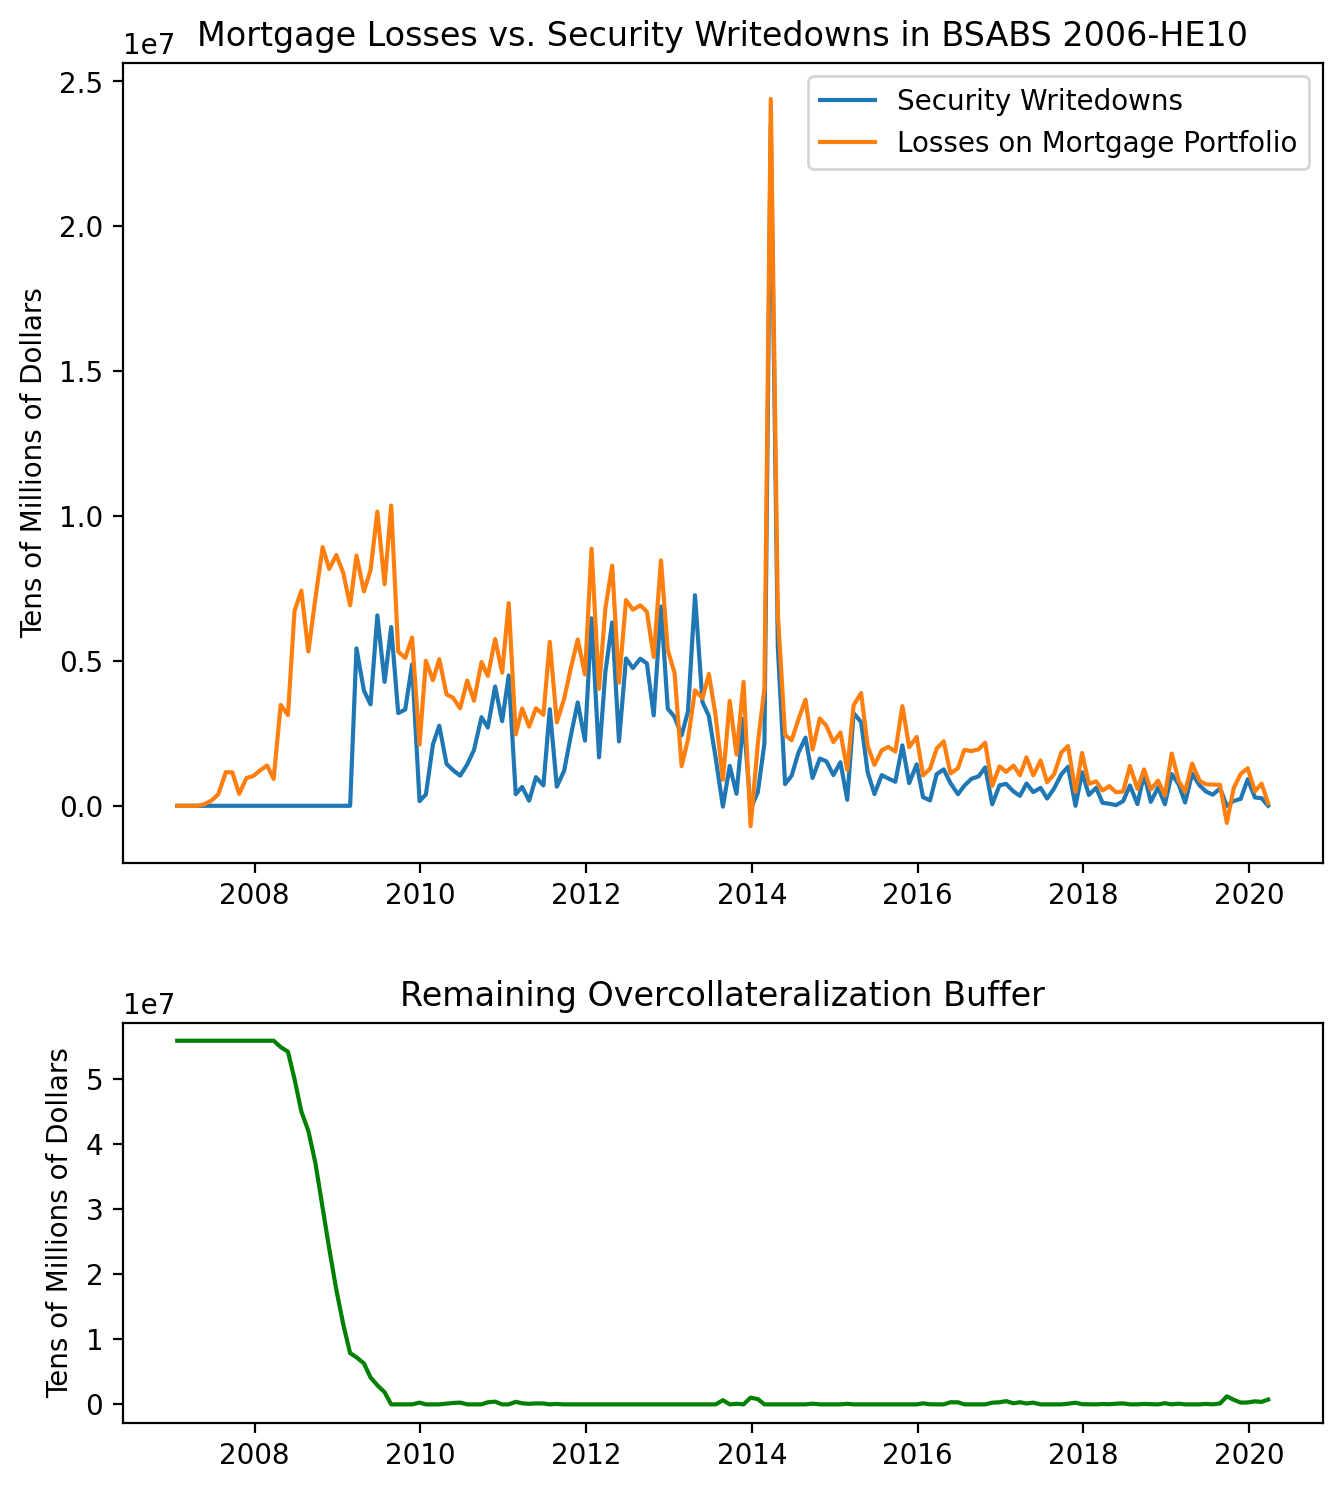
\includegraphics[width=0.8\textwidth]{../figures/timeseries_losses_vs_writedowns}
	\label{fig:timeseries_losses_vs_writedowns}
\end{figure}

At a very high level, this shows us roughly what we would expect from a poorly performing MBS deal: the overcollateralization buffer is rapidly used up in an effort to cover mortgage losses, and writedowns on the MBS’s constituent tranches rise immediately afterwards. Perhaps surprisingly, after the initial OC buffer – which represents the initial excess of the face value of the mortgages over the face value of the securities – goes to zero, there’s still a significant gap between mortgage losses from defaulting borrowers and principal losses on securities that directly affect investors. The most likely explanations for this are either excess spread due to consistent interest payments or extra cash generated by the deal’s swap agreement, so we need to figure out which effect dominated.

	Because the prospectus and other associated documents for BSABS 2006-HE10 are incredibly long and dense, it turns out that even a simple-sounding task such as trying to figure out which income streams make up the principal payments that are sent to security holders each month ends up being tough. So, it takes some time to try to piece things together from the investor reports, and even after familiarizing oneself with the intricacies of this particular bunch of securities, it’s still easy to see how anybody without an advanced finance background would view MBS deals as essentially black boxes. The data in the investor reports ultimately showed that the main sources of the cash that was sent out to investors as principal payments were 1) principal payments from the mortgages themselves, 2) interest payments from the mortgages exceeding those which had to be made to the securities, i.e. excess spread, and 3) cash coming in from the swap provider, which was negative on net. Although it’s not a perfect fit, the sum of these three components still matches up well with the series of certificate principal payments, as shown below, confirming that these are the main factors at play.

To calculate the true extent of excess spread created throughout this deal’s life, since it’s not listed on the front page of the investor reports with the other types of payments to securities, we need to know both 1) the total interest remitted from the mortgage servicer to the trust and 2) the total interest paid out to the securities each month. It turns out that from January 2007 to March 2020, the mortgages in this deal generated \$249 million of excess spread. As described in Part I, when mortgage writedowns rise, the trustee is forced to either write down one or more MBS tranches or to use excess spread (if any is present) to pay off some MBS principal. If there had been no excess spread, then in the event that the servicer had to write off some mortgage principal due to defaults, the trustee would have had no choice but to write down the lowest-rated security remaining in the deal by the full amount of the mortgage writeoffs. However, when they have some extra cash available each month due to excess spread, the trustee can make extra principal payments to the top-rated remaining security, reducing the magnitude of the monthly markdowns on the bottom tranche. As I understand it, the sequence of events each month is as follows: 

\begin{figure}[h]
	\centering
	\caption{Main Components of Principal Payments Received by Securities}
	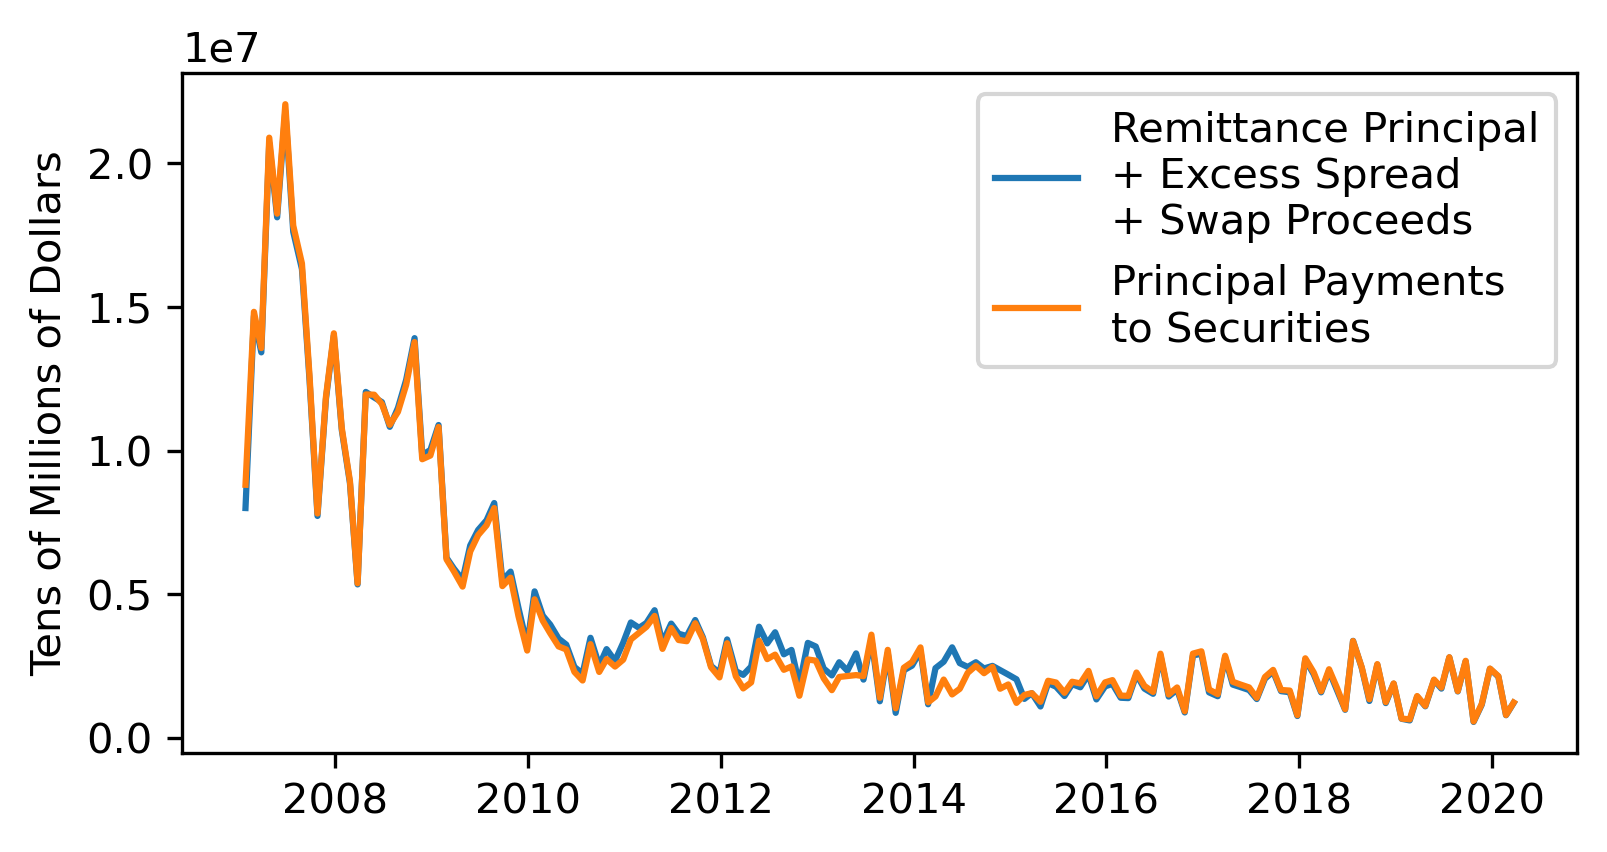
\includegraphics[width=0.8\textwidth]{../figures/timeseries_security_principal_pmts_composition}
	\label{fig:timeseries_security_principal_pmts_composition}
\end{figure}

\begin{enumerate}
	\item Borrowers make their mortgage payments
	\item The resulting principal and interest are sent to the trust
	\item Interest payments are made to securities
	\item Excess spread is calculated
	\item Excess spread is distributed as principal payments to the top MBS tranche
	\item The lowest MBS tranche is written down by the necessary amount to make up the difference between mortgage pool shrinkage and security balance shrinkage
\end{enumerate}

In the long run, even though we saw that the mortgages faced much larger principal losses than the securities, both balances saw similar total declines in principal over time: since some of the top-level securities’ principal was being directly paid off using any available cash from excess spread, only a fraction of the principal losses on the mortgages actually flowed through to the securities as writedowns. This is one feature of the deal’s history that was specifically made possible by a low-interest-rate environment: while all of the securities paid out a floating interest rate to investors, 24\% of the mortgages were fixed-rate, so when rates dropped significantly in response to the Great Recession, the fixed-rate borrowers ended up providing more interest than what needed to be paid out on the adjustable-rate securities. While this discussion of security vs. mortgage principal shrinkage may seem like nothing more than an accounting puzzle, the result of it is that we now have a clearer understanding of how important the deal’s excess spread provision was for mitigating realized losses, and we can see that it played a much larger role than the other available credit enhancement mechanism, the initial overcollateralization buffer.


\subsection*{The Swap Agreement}

In addition, at the level of the entire deal, not a single security, the final factor that influenced the extent to which investors felt the effects of poor mortgage performance was the deal’s associated swap agreement. It’s technically two separate agreements (one for Group I, one for Group II) buried under several pages of legal jargon, but the main idea is that from 2007 through 2011, the trust (the “Swap Administrator”) received floating-rate payments from Wachovia (the “Swap Provider”) while paying a fixed rate back to Wachovia. Each month, the trust paid out a rate of 4.935\% (for Group I) or 4.9315\% (for Group II) on a continually declining balance, which is the monthly “notional value” of the swap, and Wachovia sent back the one-month LIBOR rate. The overall performance of the two swap agreements is shown below:

\begin{figure}[h]
	\centering
	\caption{Performance of Swap Agreement}
	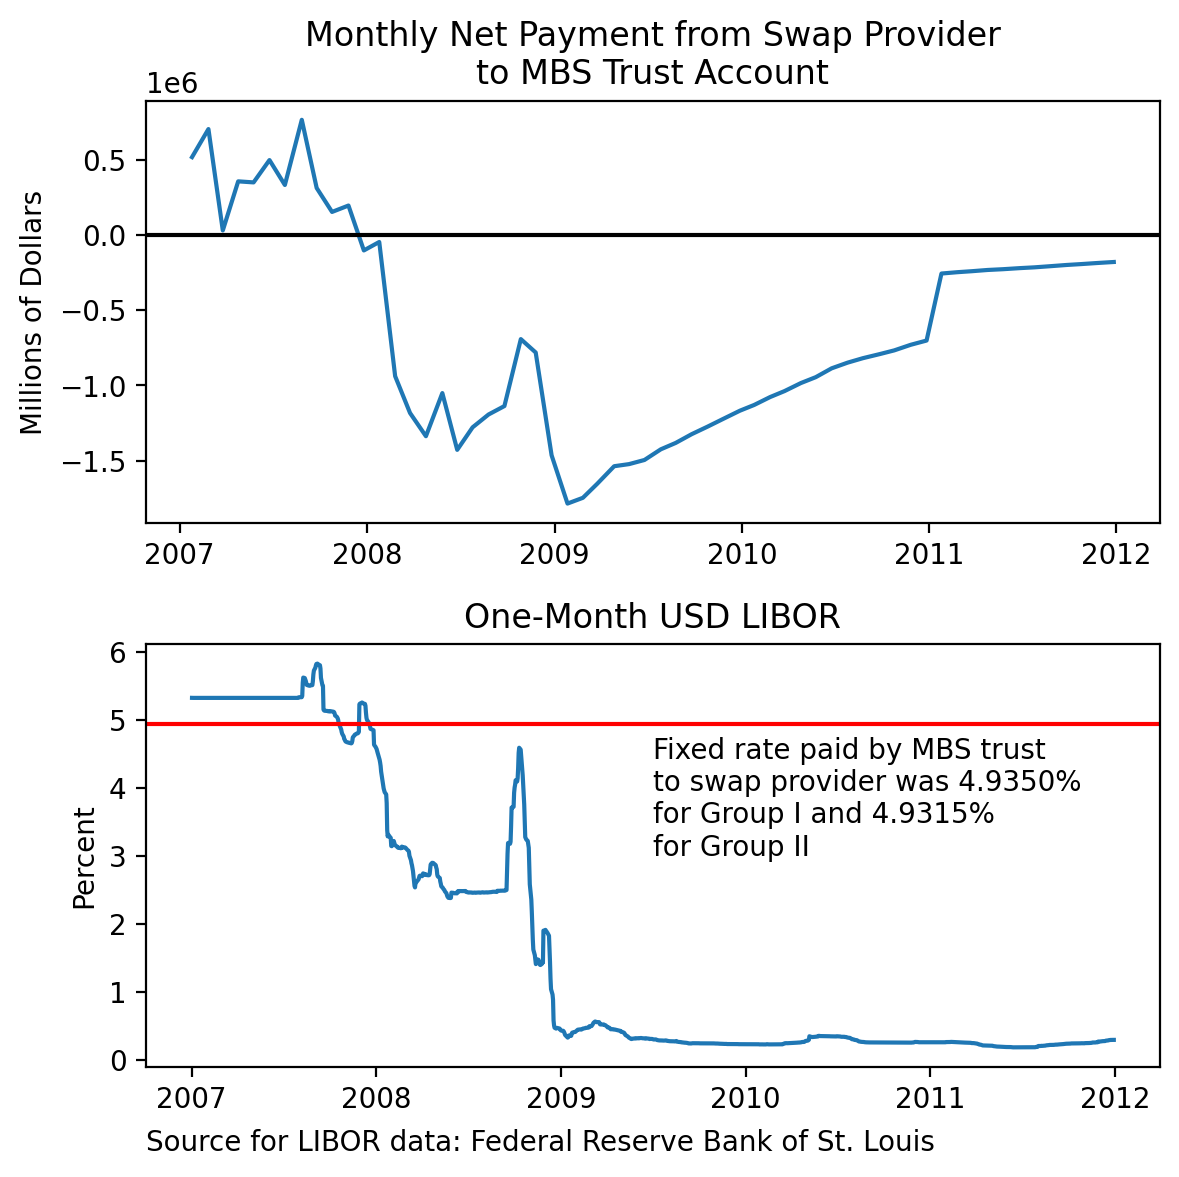
\includegraphics[width=0.8\textwidth]{../figures/timeseries_swap_performance}
	\label{fig:timeseries_swap_performance}
\end{figure}

While getting exposure to a floating-rate instrument may have seemed like a great idea in 2006 when the deal’s mortgages were being underwritten, the swap agreement turned out to be a net negative for this collection of securities. This can be seen in Figure 10, as the trust overseen by LaSalle (and then by USBank) ended up paying out millions more than it received over the life of the swap provision. Although the trends of the top and bottom graphs in Figure 10 don’t match up perfectly because the LIBOR data is provided daily and the trust only makes and receives payments once a month, this figure still clarifies the main takeaway from the swap agreement’s life, which is that receiving a floating rate and paying out a fixed rate is only beneficial if interest rates stay high. As the financial crisis worsened and central banks began cutting rates throughout 2008, LIBOR fell dramatically, which led to the net cash flow for the swap agreement being reversed – before this, the MBS trust had been profiting from receiving that floating rate, but from 2008 onward, it ended up having to use some of its monthly mortgage proceeds to pay the swap provider. On net, the trust ended up paying out approximately \$39 million to the swap provider during the swap agreement’s five-year life; while this isn’t a huge quantity compared to the overall principal balance of the deal’s securities, every dollar of that amount is still one dollar that couldn’t be distributed to investors, demonstrating a secondary way in which MBS deals can suffer when economic conditions worsen. Of course, the main channel through which a recession affects an MBS is still through mortgage defaults from borrowers being unable to make payments. However, it is also interesting to note that in a deal like this, where some of the mortgages are fixed-rate but all of the securities are floating-rate, signing a swap agreement as insurance against not being able to make interest payments to investors can backfire if global interest rates are slashed in response to a recession.


\subsection*{To What Extent Were Investors Protected From Mortgage Defaults?}

By summing up the three payment types described in Figure 9 from January 2007 to March 2020, we reach a pivotal insight about this deal’s structure, which is that on average, every \$1 of principal received by investors in this deal corresponded to approximately \$0.69 of principal payments from mortgage borrowers, \$0.37 of excess spread from borrowers’ interest payments, and -\$0.06 being sent away to the swap provider. Since it covers the entire life of the deal, not just the time before the overcollateralization buffer was completely emptied, this really highlights the importance of the excess spread mechanism for protecting investors, since a significant portion of the principal that investors received actually didn’t come from borrowers’ mortgage principal payments. The total overcollateralization buffer in this deal was roughly \$55 million at its inception in January 2007, which on its own would not have been nearly enough to significantly protect investors, given the very high volume of defaults throughout the Great Recession.

	The “principal decomposition” done above fits in nicely with another important result regarding this deal’s performance, which is that from January 2007 through March 2020, only 50.6\% of the principal writeoffs on the deal’s underlying mortgages were actually felt by investors. This is calculated by dividing the total principal markdowns for the securities by the total realized losses in the mortgage pool. This still adds up to hundreds of millions of dollars in losses for investors, but there is something to be said for the fact that the structure of this MBS protected its investors from almost half of the defaults on the assets they were exposed to.
Of course, the overall “protection rate” of 49.4\% only works at the level of the entire deal, which makes it of limited use for investors because it’s unlikely that anybody would own stakes in every single tranche for both mortgage groups. It’s worth remembering that in Group I, all of the mezzanine securities from I-M-3 down to I-M-9 were completely wiped out by writedowns, and Group II did even worse from that standpoint, with all nine II-M mezzanine tranches being written off, and II-A senior securities still taking losses today. At first glance, when you consider that more marketed securities were wiped out than were not wiped out, it looks like this deal was an absolute disaster, but as described in Part II, the mezzanine securities still made up only a small portion of the deal’s overall principal. For all the public drama surrounding super-risky mezzanine tranches and overzealous speculation on these high-yielding securities, they are still only a small proportion of the overall certificate balance of MBS deals like BSABS 2006-HE10 – the bulk of the principal is still held in the senior securities, which will take several more years to be paid off in full and have not suffered such dramatic losses.

The stratified nature of this deal does make it hard to give a single declaration as to whether investors ended up being protected from poor mortgage performance, but in my opinion, the fact that they (in the aggregate) felt barely half of the principal losses on the loans they invested in is an impressive achievement, and it’s a much better rate of protection than what I expected before I started investigating this deal in depth. The “static” overcollateralization buffer built into each deal provided only brief protection against losses during the early days of the financial crisis, but the “dynamic” mechanism of excess spread turned out to be much more important, and the prevailing low-interest-rate environment caused this second source of protection to become the dominant one for investors, as the deal ended up generating enough cash from fixed-rate interest payments to have some left over to mitigate security holders’ losses. 



\subsection*{Why Can't We Just Use Yields?}

All of this talk of whether investors in this deal were really insulated from the effects of the subprime mortgage crisis brings up another difficult-to-answer set of questions: were any of these securities actually good investments, and even more importantly, how should we be defining “good”? With more common fixed income assets like government and corporate bonds, the second of these questions is relatively easy to answer. In those cases, the bond receives interest payments each month according to some fixed coupon rate, then at the end of its maturity, the borrower makes one giant principal payment to fully pay off the face value of the bond. This gives you a convenient rough approximation for the returns you can expect from this asset: just divide the sum of one year’s coupon payments by the face value of the bond, or by the market value if it’s trading at a premium or discount to its face value. You could also use the more sophisticated measure of yield to maturity, which is the internal rate of return on the bond once you take into account all of its predicted cash flows.

	Unfortunately, neither of these metrics is readily available for the interested MBS investor, for several reasons that make estimating MBS returns challenging, including: 1) valuations for individual MBS are hard to come by, 2) each security sees its principal balance decline throughout its life, not all at once, and 3) cash flows are much more uncertain for an MBS than for a traditional bond. These three challenges manifest in the lack of an obvious market price for an MBS such as any individual tranche of BSABS 2006-HE10: because there are so many moving parts in these securities, it’s tough for anybody to make an authoritative decision about how much any one tranche is or should be worth. One can rely on the elaborate mathematical models drawn up by the issuing bank (in this case, Bear Stearns), but the resulting prices are both hard to access and of dubious validity. This exact issue is a cause of great frustration for Michael Burry in The Big Short, where it’s revealed that the daring investors like him who bet on a drop in MBS valuations had to wait long periods of time to get their payouts, because the “value” of each security was determined by the internal models of the bank that issued it, so until the bank admitted that the security was performing poorly, any short bets would not pay out. The lack of a solid market price also scrambles any attempts to predict a current yield, since the simple logic of “given a set of future annual payments C1, C2, …, what will be my yearly return on the P that I pay today?” no longer holds up when you have no idea what a reasonable price to pay for this security would be. Unfortunately. the securitization literature is relatively thin on the topic of valuation for these highly complex structured products – as Gorton and Metrick (2012) put it, “Asset pricing of ABS is woefully lacking”. Using the prices from prior transactions could be one workaround, but this still doesn’t fully solve the problem of having to constantly re-value an asset whose principal base is shrinking every month. Because of all of these issues, we’ve stuck to asking more roundabout questions like “what share of mortgage defaults actually led to security writedowns” here, rather than trying to give a single rate of return for each tranche or the deal as a whole.


\subsection*{Maiden Lane: What Happened to the Fed's Money?}

Now that we understand the extent of the connection between mortgage defaults and security writedowns, we can finally answer one of our most important questions from earlier, namely whether the Federal Reserve ended up losing any money on the two securities from this deal that it took on during the bailout of Bear Stearns, and more generally, whether those two securities really were so toxic that JPMorgan simply couldn’t bear to take them on. Specifically, we want to know whether the two tranches of this deal which were shifted onto the Fed’s books as part of the bailout of Bear Stearns caused significant losses for the government. When the New York Fed’s Maiden Lane fund was initially established, its creators assumed that some of Bear Stearns’s outstanding MBS were so volatile and toxic that JPMorgan simply could not add them to their balance sheet with the rest of Bear’s remaining assets. However, the deal to salvage what remained of Bear Stearns arose within a number of days, against the backdrop of a global financial crisis, which naturally casts some doubt on whether any in-depth analysis of Bear’s MBS holdings was actually done at the time. Now, with the benefit of hindsight, it seems quite valuable to unpack the contributions of our chosen MBS deal to the Maiden Lane fund’s performance, in order to clarify whether the assets that the Fed had to put on its books were really as risky as they were assumed to be at the time. With taxpayers’ money at stake, any significant purchase of securities by the Fed – even if this one was technically a loan made by the New York Fed to the separate Maiden Lane entity – deserves scrutiny, and looking back at the performance of the two MBS tranches discussed here will hopefully improve our understanding of the long-term ramifications of one of the federal government’s most dramatic interventions in the financial markets.

	To get started with unpacking the performance of BSABS 2006-HE10’s two Maiden Lane securities, we will lay out some summary information about the two tranches’ status at origination and their performance since 2007:

\begin{table}[h]
	\centering
	\begin{tabular}{| p{0.4\linewidth} | p{0.25\linewidth} | p{0.25\linewidth} |}
\hline
 & \textbf{I-A-3} & \textbf{II-1A-3} \\
\hline
Initial Principal Balance & \$11,213,000 & \$20,339,000 \\
\hline
Principal Payments & \$0 & \$0 \\
\hline
Interest Payments & \$2,168,104 & \$3,735,896 \\
\hline
Principal Writedowns & \$0 & \$3,705,585 \\
\hline
Initial Pass-Through Rate & 5.59\% & 5.59\% \\
\hline
Most Recent Pass-Through Rate & 1.87\% & 1.87\% \\
\hline
Initial Credit Rating (Moody’s) & Aaa & Aaa \\
\hline
Most Recent Credit Rating (Moody’s) & Baa3 (lowest investment-grade rating) & Ca (non-investment grade) \\
\hline
Principal “Loss Rate” & 0\% & 18.2\% \\
\hline
Remaining Principal Balance & \$11,213,000 & \$16,633,415 \\
\hline
\end{tabular}

	\caption{Performance Summary for Tranches I-A-3 and II-1A-3 (Data Through March 2020)}
	\label{tab:table_maiden_lane_performance}
\end{table}

\begin{figure}[h]
	\centering
	\caption{Remaining Principal Balance for Tranche I-A-3}
	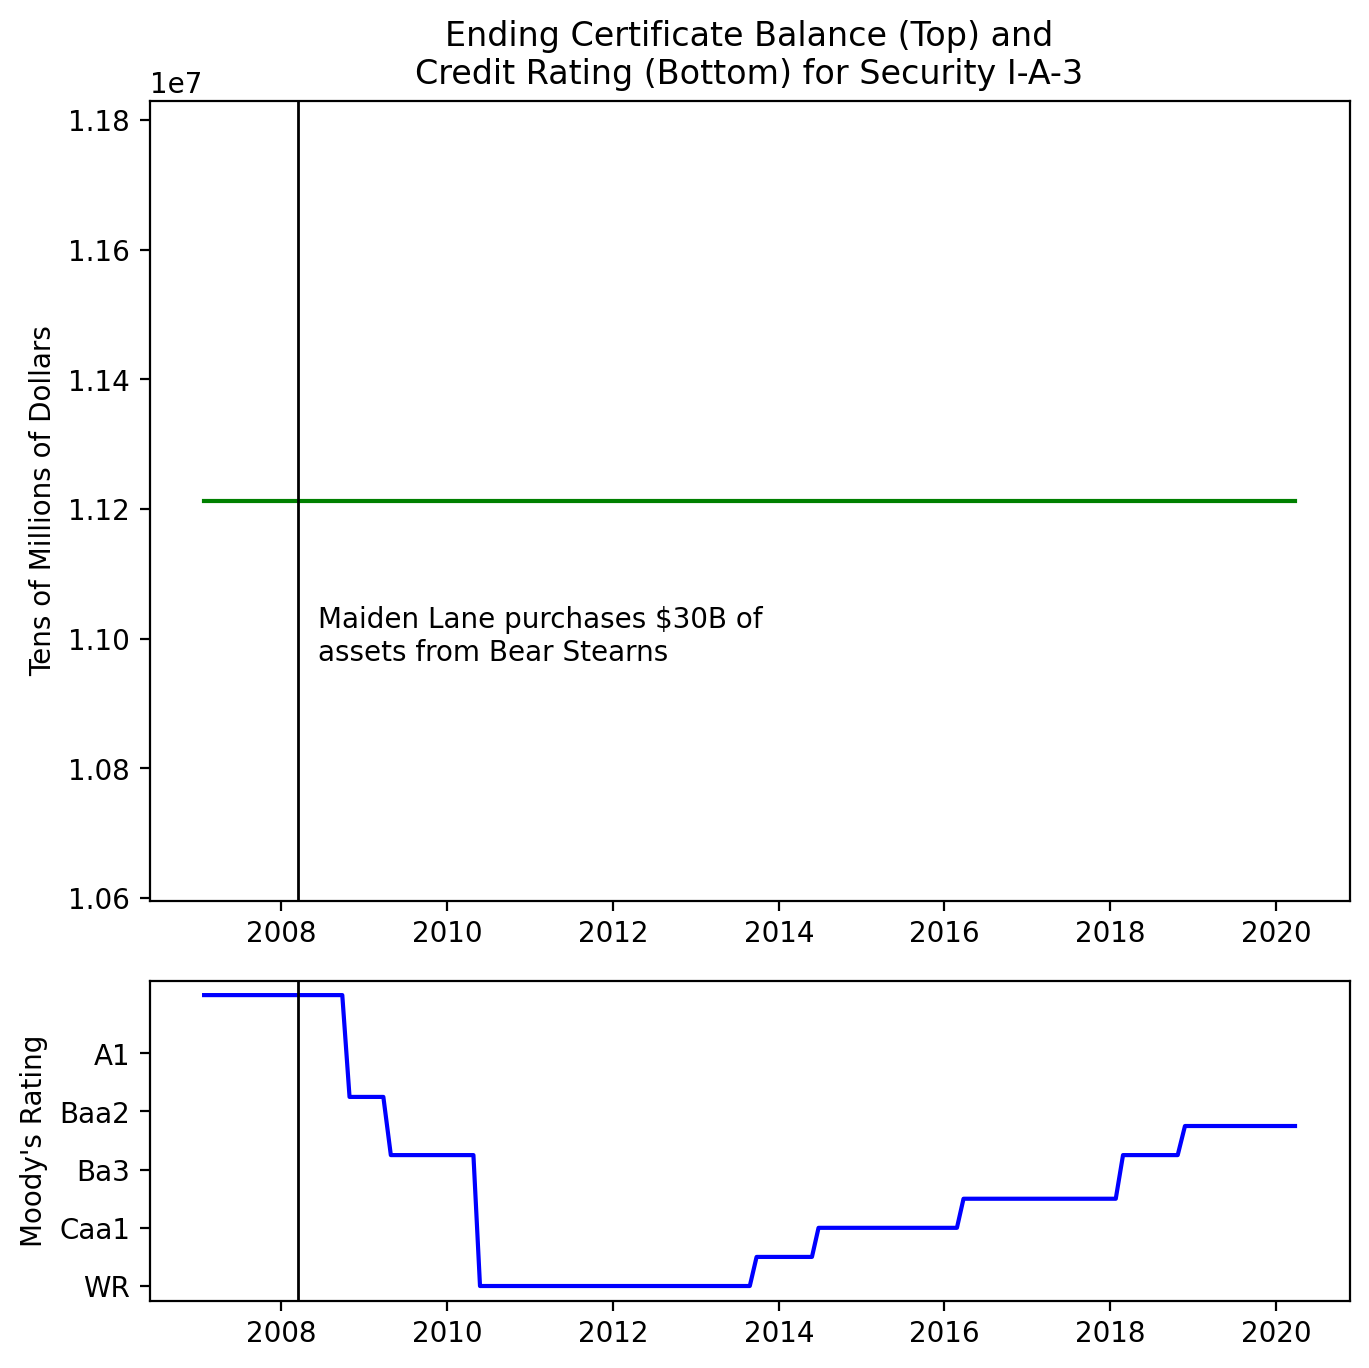
\includegraphics[width=0.8\textwidth]{../figures/timeseries_maiden_lane_ia3}
	\label{fig:timeseries_maiden_lane_ia3}
\end{figure}

\begin{figure}[h]
	\centering
	\caption{Remaining Principal Balance for Tranche II-1A-3}
	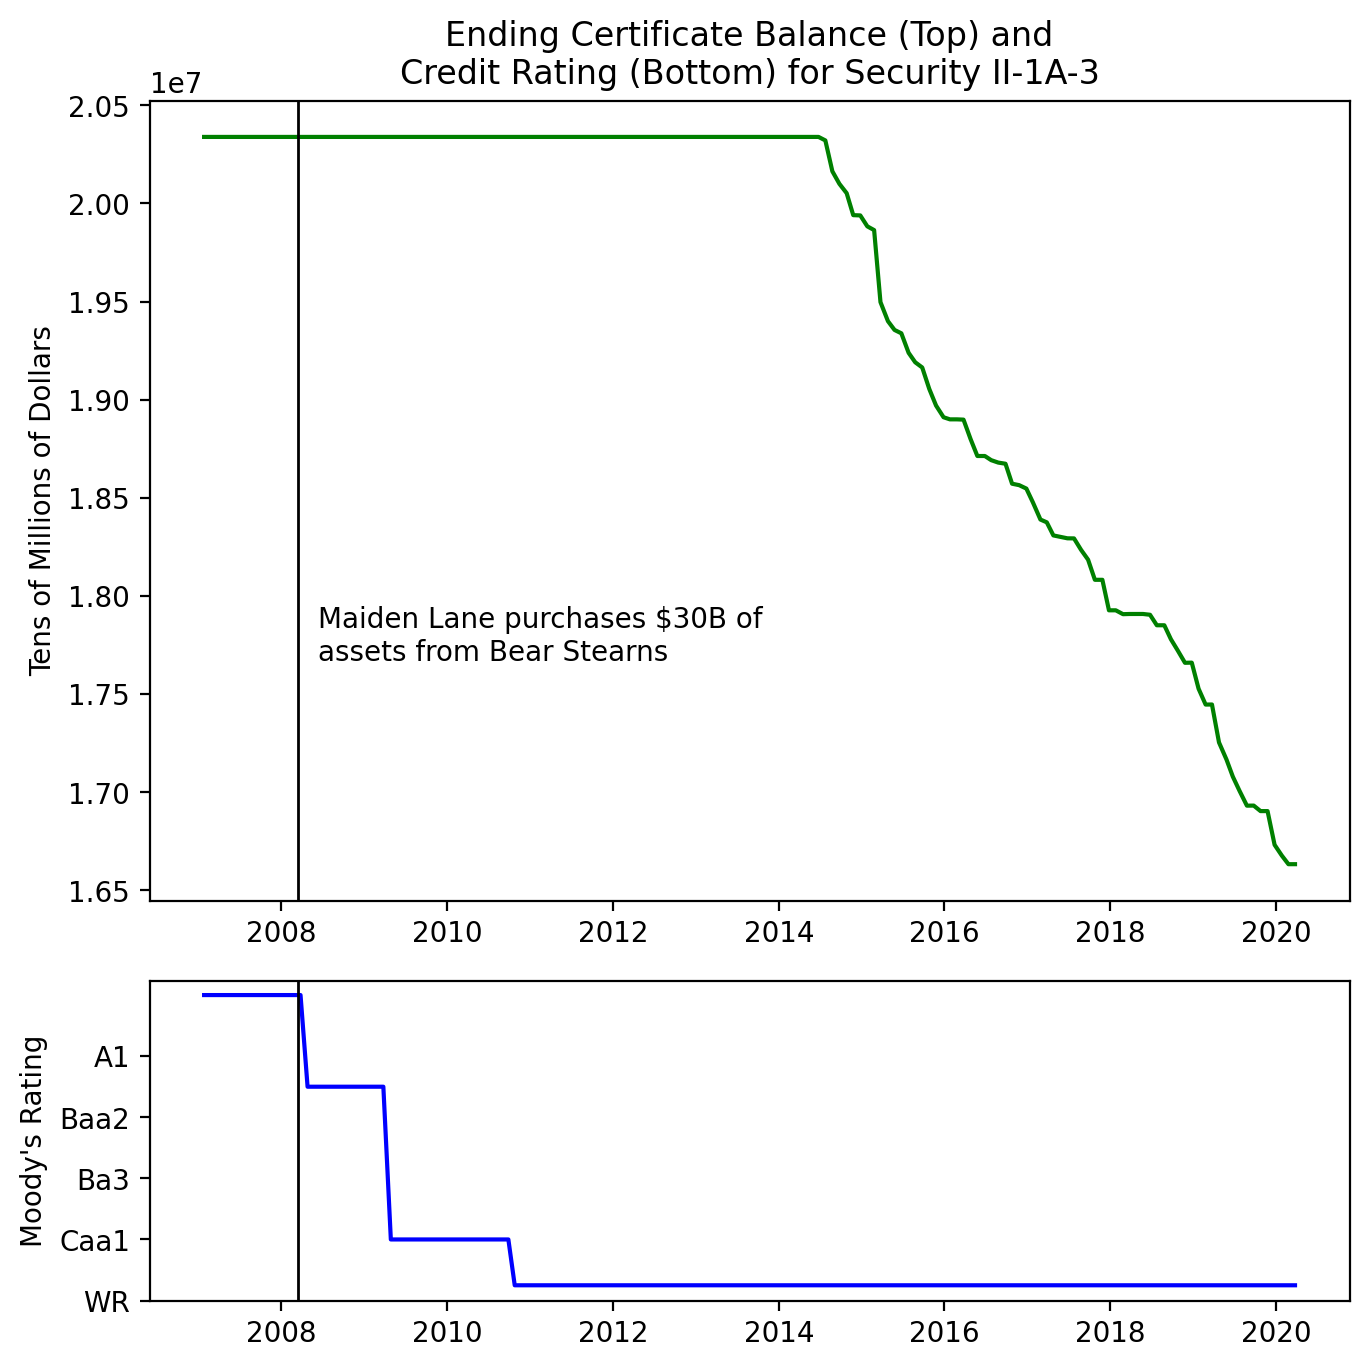
\includegraphics[width=0.8\textwidth]{../figures/timeseries_maiden_lane_ii1a3}
	\label{fig:timeseries_maiden_lane_ii1a3}
\end{figure}

As we can see in Table III and Figure 11, neither security has taken particularly heavy losses so far, although II-1A-3 is currently exposed to further writedowns because all of the mezzanine-level tranches in Group II have been fully written off already. Both securities have received significant interest payments, although this information isn’t as useful as it could be since we don’t have a clear metric for estimating rates of return. In addition, both tranches started off with perfect Aaa credit ratings, but their ratings have diverged significantly since then: I-A-3 was downgraded dramatically but has recovered its credit rating partially in recent years, while II-1A-3 has not recovered from its series of downgrades during the crisis and is still stuck in junk-bond purgatory today. The divergence in ratings is explained by the fact that I-A-3 still has mezzanine principal below it to absorb any further losses, while II-1A-3 has lost all of its subordination-based credit enhancement and is now directly exposed to future mortgage defaults.

From this brief summary, it looks like at least for this specific deal, the Fed’s purchase of Bear Stearns’s most toxic MBS assets ended up being less dangerous than expected. Since both of these securities are relatively high in the seniority hierarchy, they were well-protected from losses, although II-1A-3 was not quite as bulletproof as its original Aaa rating from 2007 implied. Overall, these securities fit solidly into the “lower senior” group described in Part II: relatively low risk of losses, but also low returns and a very long actual maturity. Going forward, we can expect these two tranches to be some of the last to be paid off in the entire deal, as they each have at least one senior security above them that would receive future principal payments first. In addition, we can also predict relatively low returns for both - and possibly negative returns for II-1A-3 if its writedowns continue - as they started off with relatively low coupon rates in 2007 (compared to the mezzanine tranches), and those pass-through rates have fallen precipitously since then.

In the chaos of a few short weeks when Bear Stearns’s situation went from bad to worse and an urgent rescue was needed, it was easy to lump these two securities in with the pile of “all subprime MBS” and assume that they were going to perform terribly, but with the benefit of over a decade of hindsight, it looks like neither of them was as dangerous as JPMorgan or the Fed assumed when the two parties agreed on how to divide up Bear’s assets. This fits in with the general trend of the Maiden Lane fund’s performance, as it only took until June 2012 for the New York Fed’s \$29B loan to Maiden Lane LLC to be fully paid off \parencite{schaefer12}. So, by looking back at this deal’s performance a few years after its most chaotic times, we’ve been able to reach the overall conclusion that the Fed’s foray into investing in BSABS 2006-HE10 ended up not being particularly toxic, which allows us to be somewhat optimistic about what would happen if a similar crisis were to occur in the future. Of course, mezzanine tranches like the ones from this deal would be a much riskier bet for the government to take on, but if future debates regarding the insolvency of major financial firms hinge on how to judge securities of roughly this caliber (lower senior), then banks and the government may want to look more closely at whether the securities in question, like I-A-3 and II-1A-3 from this deal, are really so toxic as to truly require being put into a “bad bank” by the Fed. That’s much more easily said than done, but it does give us a small benchmark for evaluating mortgage-backed securities when future financial chaos occurs – in this one case, at least, we see that these two senior-level securities which were labeled by JPMorgan Chase as highly dangerous during the height of the subprime mortgage crisis did not completely collapse, and in fact performed reasonably well, if not spectacularly so.


\section*{Conclusion}

We’ve now discussed at length the two main elements of this securitization – the mortgages that were bundled together and generated principal and interest payments for investors, and the securities that investors actually bought. They are closely related, but we saw that these two pools of assets performed very differently, with the deal’s credit enhancement mechanisms frequently cushioning the blows felt by investors when borrowers defaulted; mezzanine investors did, though, suffer significant losses. On top of what we’ve learned about this deal’s idiosyncrasies, our analysis of how its component parts weathered the 2007-08 financial crisis and subsequent slow economic recovery also adds to the more general study of securitization and its role in the financial system. Economists have gone to great lengths to characterize the incentive structures that arise when banks securitize their loans, and the theory is valuable for understanding the ways in which stakeholders could potentially mislead others and thereby affect the deal’s performance, but it is also helpful to get our hands on some actual data and understand how well a real-life securitization responded to a severe economic crisis.

Given its large principal base ($>$\$1B) and multiple methods of credit enhancement, BSABS 2006-HE10 looks to be a good test case for studying mortgage-backed securities in general, as its tranches’ collective performance illustrates the diversity of risk levels that one can choose from when an investor purchases part of an MBS. In a partial vindication of the senior tranches’ original AAA ratings, the top security in Group I has not yet lost any principal, but the top tranches in Group II have actually suffered some losses, showing that the appraisals of credit risk provided by ratings were not as accurate as we might have hoped. At the bottom of the totem pole, investors in mezzanine tranches were more or less cleaned out, as they bet big to take advantage of high potential interest rates (coupons on the most junior tranches were above 7\% at the deal’s inception) but were subsequently burned when macroeconomic conditions took a nosedive. Squeezed in between these high-risk and low-risk segments are securities like I-A-3 and II-1A-3, those that ended up on Maiden Lane’s balance sheet during the dissolution of Bear Stearns, which have both served as great examples of the “lower senior” segment that offers neither near-guaranteed return of principal nor high potential returns. Principal losses have been zero for the former and moderate for the latter, coupon rates on the two tranches have stayed stubbornly low, and we learned that by mid-2012, the fund had sold both of these tranches and had managed to fully pay off, with interest, the loan it got from the New York Fed for purchasing these assets and others. Any financial asset that was purchased with taxpayer money deserves a high degree of scrutiny, and in this particular case, it looks like Maiden Lane got away with purchasing two tranches which were much less toxic than analysts believed during the chaotic weeks leading up to JPMorgan Chase’s takeover of Bear Stearns.


\subsection*{MBS-Related Lawsuits Against Bear Stearns}

Although we saw that the Fed’s purchase of assorted MBS from Bear Stearns’s ended up yielding profits for the government, the debate over whether securities such as those in BSABS 2006-HE10 were appropriate for the general population of investors gets more complicated when we recall the lawsuits filed against Bear Stearns which included this deal in their lists of relevant securities. The most important of these was a suit filed by the Department of Justice against JPMorgan Chase, which assumed responsibility for MBS products issued by Bear Stearns and Washington Mutual as well as its own MBS issuances. The DOJ’s investigation – which did officially reference BSABS 2006-HE10 – uncovered the fact that Bear Stearns executives sometimes deliberately ignored statements from loan originators about how new loans did not meet the originators’ underwriting guidelines, choosing to purchase those loans for MBS deals anyway (DOJ 2013). In addition, after disqualifying certain mortgage originators from contributing loans for future securitizations due to consistently poor mortgage performance, Bear Stearns bankers failed to actually re-examine or repurchase those sellers’ low-quality loans which were already present in Bear Stearns-issued MBS, marking another example of how the bank failed to inform investors that the mortgages they were investing in were weaker than what they were promised (DOJ 2013). Ultimately, JPMorgan was forced to admit that it had made “serious misrepresentations” to investors by securitizing loans that did not meet advertised underwriting guidelines, and it was required to pay out a total of \$13 billion. This consisted of a \$2 billion fine for JPMorgan’s own activities, \$4 billion in various forms of debt relief for homeowners whose mortgages had been securitized, and most of the remainder going to the FHFA and other large investors who had bought questionable securities issued by Bear Stearns, Washington Mutual and JPMorgan itself \parencite{eavis13}. 

In a separate complaint by the SEC against several Bear Stearns-related defendants, including Bear Stearns Asset-Backed Securities I LLC, the entity that issued deals such as BSABS 2006-HE10, it was also revealed that Bear Stearns failed to pressure originators to re-purchase bad loans from MBS trusts if the loans missed any payments in the deal’s first three months, which was a provision in many deals’ prospectuses. Instead of requiring the originator to buy back each severely delinquent loan, Bear Stearns would often accept a bulk payment from the cash-strapped originator to address many delinquencies at once, and would then hold that cash on its own books, while leaving those low-quality loans remaining in the mortgage pools of the MBS that it had sold to investors (Securities and Exchange Commission v. J.P. Morgan Securities LLC et. al 2013). The initial complaint and final court judgment from that case, which resulted in a \$222 million penalty for the defendants, don’t mention whether this practice specifically occurred for BSABS 2006-HE10, but it’s still highly concerning that this much misconduct was going on in the vicinity of deals such as the one we examined here.

On top of the scrutiny it faced from the federal government, JPMorgan ended up having to answer yet again for its own questionable MBS-related practices, not just the issues it inherited from Bear Stearns. A few years after the crisis, JPMorgan was sued by several large institutional investors on behalf of their clients, alleging that the bank’s mortgage servicing practices did not live up to the standards laid out in the Pooling and Servicing Agreements that covered many deals originated by Bear Stearns and JPMorgan itself \parencite{gibbs13}. In 2013, JPMorgan agreed to pay \$4.5 billion to various MBS trustees to settle these claims, and it also committed to making several improvements to its servicing practices. In particular, BSABS 2006-HE10 acquired another stain on its record by being officially cited in the list of securities covered by the settlement.


\subsection*{What Comes Next for Securitization}

To finish off our consideration of this deal’s legacy, we should also consider how the world of securitization has changed since the Great Recession, and how new regulations might affect future deals like this one. To remedy some of the moral hazard present in the securitization process, US regulations now require the issuer of a securitized product to retain no less than 5\% of its credit risk, either by owning 5\% of each tranche or by owning the first-loss (bottom) tranche as well as enough of the other securities to reach a total of 5\% \parencite{scheicher17}. Other new rules have also introduced more elaborate capital requirements, and dramatically higher (compared to pre-crisis regulations) weightings for securitizations in the risk-weighted capital tests that are used to judge banks’ degrees of leverage \parencite{scheicher17}. In reality, these new regulations have so far been applied to a much-diminished market: \textcite{gorton12} point out that the 2007-08 crisis put an almost complete halt to new asset-backed securities issuance. Both sell-side and buy-side arguments could potentially explain this. One the side of MBS issuers, the credit crunch after the 2007 housing crash, and the associated tightening of lending standards, would have dramatically reduced the number of new loans available to be securitized. In addition, it would not be surprising if investors had become much more suspicious of the complex instruments that they had previously been eager to buy, and they may have also been responding to the new public stigma surrounding mortgage-backed securities that resulted from these assets’ role in the crisis. Either way, the new suite of regulations hit an asset class that is to this day still trying to regain its pre-recession role in the global financial markets.

Since the crisis, there has been significant research activity aimed at refining our understanding of where the securitization process can go wrong, with a lot of attention on the massive role that credit ratings play in helping investors decide whether to buy an MBS or any other type of asset-backed security. As just one example, \textcite{efing14} found that credit rating agencies were more likely to give high ratings to deals issued by firms that they did a lot of business with, providing evidence that significant conflicts of interest could lead to the distribution of inflated credit ratings for mediocre securities. This seems like a compelling argument when we consider the fact that every single marketed tranche of BSABS 2006-HE10 received an investment-grade rating at the deal’s inception in 2007, despite the fact that the lower tranches had minimal subordination protection; as we saw, most of the mezzanine tranches would go on to be completely wiped out thanks to principal writedowns. Results like that of Efing and Hau were behind the post-recession efforts of global standards-setting bodies like the Financial Stability Board to find ways to lessen investors’ dependence on credit ratings for evaluating MBS, but this shift has not happened fully and will probably be quite difficult. Even several years before the financial crisis, it was well known that credit rating agencies were fundamentally tied into the world of securitization. According to Fitch Ratings’s then-vice chairman Neil Baron in his 1998 contribution to the book A Primer on Securitization, “Without ratings, the complex securities in the mortgage field which rely so heavily on the strength of credit enhancements might not be able to be sold” \parencite{baron98}. This quip would very likely apply to the tranches of something like BSABS 2006-HE10, since its multiple credit enhancement mechanisms added to the already-present challenge of doing credit analysis on a product made up of thousands of individual loans. Even coming from a ratings agency executive who had a lot to gain from making his ratings seem as important as possible, it is still concerning to hear that opaque credit ratings play such an instrumental role in the basic process of securitization, and this implies that giving investors ways to avoid fixating on opaque credit ratings when choosing which MBS to invest in will be a great challenge. Some progress has been made, but there is still more that needs to be done to make this aspect of the securitization process less vulnerable to misconduct in the future \parencite{scheicher17}.

In conclusion, this deal offers a wide variety of insights into the practice of securitization during the height of its popularity, and its performance during the financial crisis shows us that credit enhancement mechanisms really did protect investors, but also that once defaults begin to accumulate at a sufficient pace, even the best credit enhancement techniques can’t fully prevent realized losses on an MBS deal’s lower tranches. Because the data used in this report only cover January 2007 through March 2020, a promising future area of research would be to examine how well BSABS 2006-HE10 and similar deals have responded to the COVID-19 pandemic, a broad macroeconomic shock that has put financial pressure on mortgage borrowers nationwide. If it turns out that defaults have spiked once again, investors may be stuck with even faster writeoffs of their precious principal, which could potentially make MBS look even less appealing going forward – the senior-level securities may have mostly weathered the Great Recession, but could they survive another economic crisis without completely collapsing? In theory, these securities will still be making payments until 2036, so much more loan-related and deal-related data will be produced in the coming years, and hopefully this deal will continue to serve as a valuable example for studying how mortgage-backed securities perform in times both good and bad.

\newpage

\nocite{*}
\printbibliography

\newpage
\section*{Appendix A: Deal Structure}
\begin{figure}[h]
	\centering
	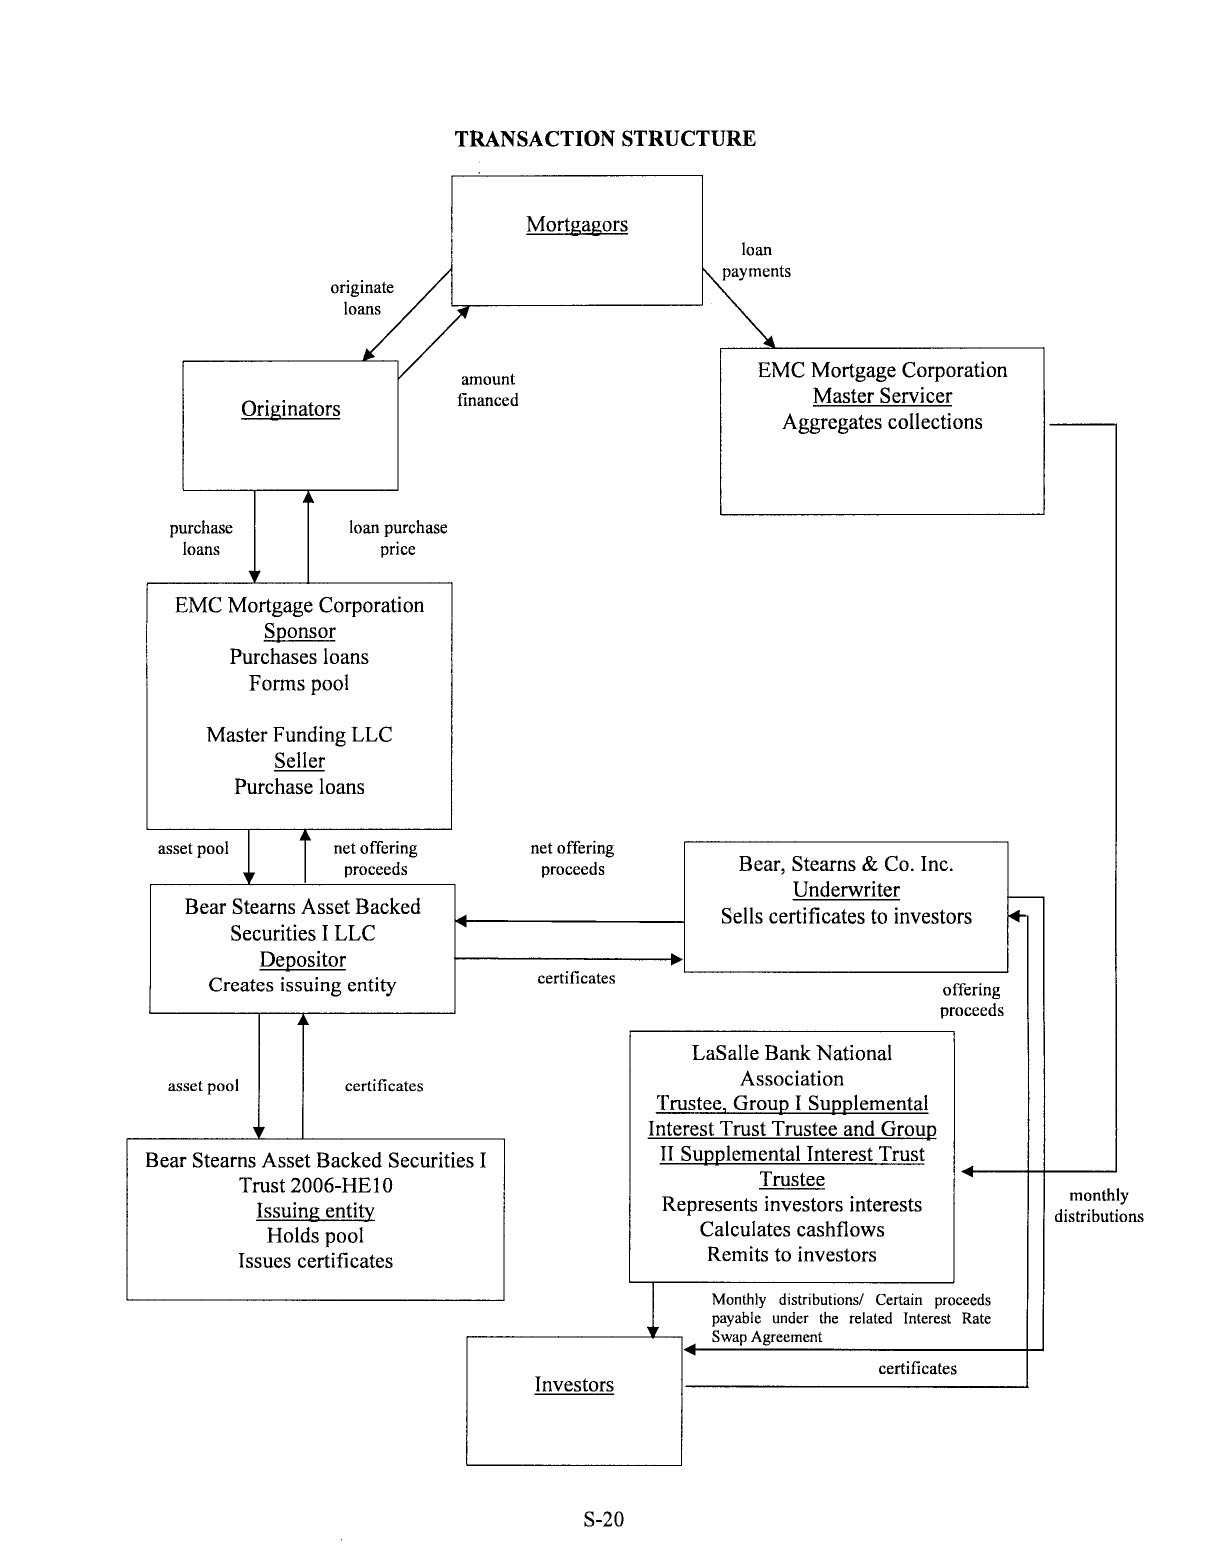
\includegraphics[width=0.9\textwidth]{../figures/deal_structure_from_prospectus}
\end{figure}


\newpage

\begin{landscape}
\section*{Appendix B: Mortgage Performance by Loan Type (through May 2013)}

\begin{longtable}{|p{0.2\linewidth}|p{0.1\linewidth}|p{0.15\linewidth}|p{0.1\linewidth}|p{0.2\linewidth}|p{0.2\linewidth}|}
\hline
Group & \textbf{Number of Loans (March 2007)} & \textbf{Principal Balance (March 2007)} & \textbf{Loss Rate (baseline is March 2007)} & \textbf{Share of March 2007 Principal} & \textbf{Share of All Realized Losses (January 2007-May 2013)} \\
\hline
Total (All Loans)                          &                        5,073 &                 \$1,114,950,509 &                              31.4\% &                        100.0\% &                                             100.0\% \\
\hline
ARM                                        &                        3,405 &                   \$847,195,525 &                              32.0\% &                         76.0\% &                                              77.3\% \\
\hline
Fixed                                      &                        1,668 &                   \$267,754,984 &                              29.8\% &                         24.0\% &                                              22.7\% \\
\hline
Group I                                    &                        1,522 &                   \$313,081,396 &                              28.8\% &                         28.1\% &                                              25.7\% \\
\hline
Group I Loans 228 ARM                      &                        1,094 &                   \$248,404,264 &                              29.7\% &                         22.3\% &                                              21.1\% \\
\hline
Group I Loans 327 ARM                      &                           38 &                     \$8,230,611 &                              17.5\% &                          0.7\% &                                               0.4\% \\
\hline
Group I Loans Fixed 1st Lien               &                          284 &                    \$50,617,127 &                              19.8\% &                          4.5\% &                                               2.9\% \\
\hline
Group I Loans Fixed 2nd Lien               &                          106 &                     \$5,829,394 &                              83.1\% &                          0.5\% &                                               1.4\% \\
\hline
Group II                                   &                        3,551 &                   \$801,869,113 &                              32.5\% &                         71.9\% &                                              74.3\% \\
\hline
Group II Loans Subgroup I 228 ARM          &                          787 &                   \$253,703,351 &                              34.9\% &                         22.8\% &                                              25.2\% \\
\hline
Group II Loans Subgroup I 327 ARM          &                           92 &                    \$28,497,466 &                              35.7\% &                          2.6\% &                                               2.9\% \\
\hline
Group II Loans Subgroup I Fixed 1st Lien   &                          273 &                    \$66,556,174 &                              22.1\% &                          6.0\% &                                               4.2\% \\
\hline
Group II Loans Subgroup I Fixed 2nd Lien   &                          393 &                    \$29,495,741 &                              85.9\% &                          2.6\% &                                               7.2\% \\
\hline
Group II Loans Subgroup II 228 ARM         &                          709 &                   \$161,584,502 &                              31.8\% &                         14.5\% &                                              14.7\% \\
\hline
Group II Loans Subgroup II 327 ARM         &                           98 &                    \$21,965,710 &                              30.8\% &                          2.0\% &                                               1.9\% \\
\hline
Group II Loans Subgroup II Fixed 1st Lien  &                          343 &                    \$69,912,843 &                              19.7\% &                          6.3\% &                                               3.9\% \\
\hline
Group II Loans Subgroup II Fixed 2nd Lien  &                           66 &                     \$3,254,755 &                              78.6\% &                          0.3\% &                                               0.7\% \\
\hline
Group II Loans Subgroup III 228 ARM        &                          491 &                   \$110,952,995 &                              32.0\% &                         10.0\% &                                              10.1\% \\
\hline
Group II Loans Subgroup III 327 ARM        &                           96 &                    \$13,856,626 &                              23.7\% &                          1.2\% &                                               0.9\% \\
\hline
Group II Loans Subgroup III Fixed 1st Lien &                          203 &                    \$42,088,950 &                              20.0\% &                          3.8\% &                                               2.4\% \\
\hline
\end{longtable}

\end{landscape}

\end{document}



